\documentclass[twoside]{book}

% Packages required by doxygen
\usepackage{calc}
\usepackage{doxygen}
\usepackage{graphicx}
\usepackage[utf8]{inputenc}
\usepackage{makeidx}
\usepackage{multicol}
\usepackage{multirow}
\usepackage{textcomp}
\usepackage[table]{xcolor}

% Font selection
\usepackage[T1]{fontenc}
\usepackage{mathptmx}
\usepackage[scaled=.90]{helvet}
\usepackage{courier}
\usepackage{amssymb}
\usepackage{sectsty}
\renewcommand{\familydefault}{\sfdefault}
\allsectionsfont{%
  \fontseries{bc}\selectfont%
  \color{darkgray}%
}
\renewcommand{\DoxyLabelFont}{%
  \fontseries{bc}\selectfont%
  \color{darkgray}%
}

% Page & text layout
\usepackage{geometry}
\geometry{%
  a4paper,%
  top=2.5cm,%
  bottom=2.5cm,%
  left=2.5cm,%
  right=2.5cm%
}
\tolerance=750
\hfuzz=15pt
\hbadness=750
\setlength{\emergencystretch}{15pt}
\setlength{\parindent}{0cm}
\setlength{\parskip}{0.2cm}
\makeatletter
\renewcommand{\paragraph}{%
  \@startsection{paragraph}{4}{0ex}{-1.0ex}{1.0ex}{%
    \normalfont\normalsize\bfseries\SS@parafont%
  }%
}
\renewcommand{\subparagraph}{%
  \@startsection{subparagraph}{5}{0ex}{-1.0ex}{1.0ex}{%
    \normalfont\normalsize\bfseries\SS@subparafont%
  }%
}
\makeatother

% Headers & footers
\usepackage{fancyhdr}
\pagestyle{fancyplain}
\fancyhead[LE]{\fancyplain{}{\bfseries\thepage}}
\fancyhead[CE]{\fancyplain{}{}}
\fancyhead[RE]{\fancyplain{}{\bfseries\leftmark}}
\fancyhead[LO]{\fancyplain{}{\bfseries\rightmark}}
\fancyhead[CO]{\fancyplain{}{}}
\fancyhead[RO]{\fancyplain{}{\bfseries\thepage}}
\fancyfoot[LE]{\fancyplain{}{}}
\fancyfoot[CE]{\fancyplain{}{}}
\fancyfoot[RE]{\fancyplain{}{\bfseries\scriptsize Generated on Mon May 6 2019 18\-:45\-:43 for Game\-Logic by Doxygen }}
\fancyfoot[LO]{\fancyplain{}{\bfseries\scriptsize Generated on Mon May 6 2019 18\-:45\-:43 for Game\-Logic by Doxygen }}
\fancyfoot[CO]{\fancyplain{}{}}
\fancyfoot[RO]{\fancyplain{}{}}
\renewcommand{\footrulewidth}{0.4pt}
\renewcommand{\chaptermark}[1]{%
  \markboth{#1}{}%
}
\renewcommand{\sectionmark}[1]{%
  \markright{\thesection\ #1}%
}

% Indices & bibliography
\usepackage{natbib}
\usepackage[titles]{tocloft}
\setcounter{tocdepth}{3}
\setcounter{secnumdepth}{5}
\makeindex

% Hyperlinks (required, but should be loaded last)
\usepackage{ifpdf}
\ifpdf
  \usepackage[pdftex,pagebackref=true]{hyperref}
\else
  \usepackage[ps2pdf,pagebackref=true]{hyperref}
\fi
\hypersetup{%
  colorlinks=true,%
  linkcolor=blue,%
  citecolor=blue,%
  unicode%
}

% Custom commands
\newcommand{\clearemptydoublepage}{%
  \newpage{\pagestyle{empty}\cleardoublepage}%
}


%===== C O N T E N T S =====

\begin{document}

% Titlepage & ToC
\hypersetup{pageanchor=false}
\pagenumbering{roman}
\begin{titlepage}
\vspace*{7cm}
\begin{center}%
{\Large Game\-Logic }\\
\vspace*{1cm}
{\large Generated by Doxygen 1.8.6}\\
\vspace*{0.5cm}
{\small Mon May 6 2019 18:45:43}\\
\end{center}
\end{titlepage}
\clearemptydoublepage
\tableofcontents
\clearemptydoublepage
\pagenumbering{arabic}
\hypersetup{pageanchor=true}

%--- Begin generated contents ---
\chapter{Main Page}
\label{index}\hypertarget{index}{}\href{https://travis-ci.org/SoPra-Team-10/GameLogic}{\tt !\mbox{[}Build Status\mbox{]}(https\-://travis-\/ci.\-org/\-So\-Pra-\/\-Team-\/10/\-Game\-Logic.\-svg?branch=master)}

Die Spiellogik u.\-a. für den Server

\subsection*{Installing}

First you need to install \href{https://github.com/SoPra-Team-10/Messages}{\tt Sopra\-Message}.

In the root directory of the project run ``` sudo make install ``` the library can now be included using

``` \#include $<$Sopra\-Game\-Logic/\-X\-Y$>$ ```

and linked using

``` -\/l\-Sopra\-Game\-Logic ```

\subsection*{Docu}


\begin{DoxyItemize}
\item \href{https://sopra-team-10.github.io/GameLogic/master/html/index.html}{\tt Master Brnach Docu}
\item \href{https://sopra-team-10.github.io/GameLogic/Develop/html/index.html}{\tt Develop Branch Docu} 
\end{DoxyItemize}
\chapter{Hierarchical Index}
\section{Class Hierarchy}
This inheritance list is sorted roughly, but not completely, alphabetically\-:\begin{DoxyCompactList}
\item \contentsline{section}{game\-Controller\-:\-:Action}{\pageref{classgame_controller_1_1_action}}{}
\begin{DoxyCompactList}
\item \contentsline{section}{game\-Controller\-:\-:Move}{\pageref{classgame_controller_1_1_move}}{}
\item \contentsline{section}{game\-Controller\-:\-:Shot}{\pageref{classgame_controller_1_1_shot}}{}
\end{DoxyCompactList}
\item \contentsline{section}{game\-Model\-:\-:Config}{\pageref{classgame_model_1_1_config}}{}
\item \contentsline{section}{game\-Model\-:\-:Environment}{\pageref{classgame_model_1_1_environment}}{}
\item \contentsline{section}{game\-Model\-:\-:Fanblock}{\pageref{classgame_model_1_1_fanblock}}{}
\item \contentsline{section}{game\-Model\-:\-:Foul\-Detection\-Probs}{\pageref{structgame_model_1_1_foul_detection_probs}}{}
\item \contentsline{section}{game\-Model\-:\-:Game\-Dynamics\-Probs}{\pageref{structgame_model_1_1_game_dynamics_probs}}{}
\item \contentsline{section}{game\-Controller\-:\-:Interference}{\pageref{classgame_controller_1_1_interference}}{}
\begin{DoxyCompactList}
\item \contentsline{section}{game\-Controller\-:\-:Impulse}{\pageref{classgame_controller_1_1_impulse}}{}
\item \contentsline{section}{game\-Controller\-:\-:Ranged\-Attack}{\pageref{classgame_controller_1_1_ranged_attack}}{}
\item \contentsline{section}{game\-Controller\-:\-:Snitch\-Push}{\pageref{classgame_controller_1_1_snitch_push}}{}
\item \contentsline{section}{game\-Controller\-:\-:Teleport}{\pageref{classgame_controller_1_1_teleport}}{}
\end{DoxyCompactList}
\item \contentsline{section}{game\-Model\-:\-:Object}{\pageref{classgame_model_1_1_object}}{}
\begin{DoxyCompactList}
\item \contentsline{section}{game\-Model\-:\-:Ball}{\pageref{classgame_model_1_1_ball}}{}
\begin{DoxyCompactList}
\item \contentsline{section}{game\-Model\-:\-:Bludger}{\pageref{classgame_model_1_1_bludger}}{}
\item \contentsline{section}{game\-Model\-:\-:Quaffle}{\pageref{classgame_model_1_1_quaffle}}{}
\item \contentsline{section}{game\-Model\-:\-:Snitch}{\pageref{classgame_model_1_1_snitch}}{}
\end{DoxyCompactList}
\item \contentsline{section}{game\-Model\-:\-:Player}{\pageref{classgame_model_1_1_player}}{}
\begin{DoxyCompactList}
\item \contentsline{section}{game\-Model\-:\-:Beater}{\pageref{classgame_model_1_1_beater}}{}
\item \contentsline{section}{game\-Model\-:\-:Chaser}{\pageref{classgame_model_1_1_chaser}}{}
\item \contentsline{section}{game\-Model\-:\-:Keeper}{\pageref{classgame_model_1_1_keeper}}{}
\item \contentsline{section}{game\-Model\-:\-:Seeker}{\pageref{classgame_model_1_1_seeker}}{}
\end{DoxyCompactList}
\end{DoxyCompactList}
\item \contentsline{section}{game\-Model\-:\-:Position}{\pageref{structgame_model_1_1_position}}{}
\item \contentsline{section}{game\-Model\-:\-:Team}{\pageref{classgame_model_1_1_team}}{}
\item \contentsline{section}{game\-Model\-:\-:Timeouts}{\pageref{structgame_model_1_1_timeouts}}{}
\item \contentsline{section}{game\-Model\-:\-:Vector}{\pageref{classgame_model_1_1_vector}}{}
\end{DoxyCompactList}

\chapter{Data Structure Index}
\section{Data Structures}
Here are the data structures with brief descriptions\-:\begin{DoxyCompactList}
\item\contentsline{section}{\hyperlink{classgame_controller_1_1_action}{game\-Controller\-::\-Action} }{\pageref{classgame_controller_1_1_action}}{}
\item\contentsline{section}{\hyperlink{classgame_model_1_1_ball}{game\-Model\-::\-Ball} }{\pageref{classgame_model_1_1_ball}}{}
\item\contentsline{section}{\hyperlink{classgame_model_1_1_beater}{game\-Model\-::\-Beater} }{\pageref{classgame_model_1_1_beater}}{}
\item\contentsline{section}{\hyperlink{classgame_model_1_1_bludger}{game\-Model\-::\-Bludger} }{\pageref{classgame_model_1_1_bludger}}{}
\item\contentsline{section}{\hyperlink{classgame_model_1_1_chaser}{game\-Model\-::\-Chaser} }{\pageref{classgame_model_1_1_chaser}}{}
\item\contentsline{section}{\hyperlink{classgame_model_1_1_config}{game\-Model\-::\-Config} }{\pageref{classgame_model_1_1_config}}{}
\item\contentsline{section}{\hyperlink{classgame_model_1_1_environment}{game\-Model\-::\-Environment} }{\pageref{classgame_model_1_1_environment}}{}
\item\contentsline{section}{\hyperlink{classgame_model_1_1_fanblock}{game\-Model\-::\-Fanblock} }{\pageref{classgame_model_1_1_fanblock}}{}
\item\contentsline{section}{\hyperlink{structgame_model_1_1_foul_detection_probs}{game\-Model\-::\-Foul\-Detection\-Probs} }{\pageref{structgame_model_1_1_foul_detection_probs}}{}
\item\contentsline{section}{\hyperlink{structgame_model_1_1_game_dynamics_probs}{game\-Model\-::\-Game\-Dynamics\-Probs} }{\pageref{structgame_model_1_1_game_dynamics_probs}}{}
\item\contentsline{section}{\hyperlink{classgame_controller_1_1_impulse}{game\-Controller\-::\-Impulse} }{\pageref{classgame_controller_1_1_impulse}}{}
\item\contentsline{section}{\hyperlink{classgame_controller_1_1_interference}{game\-Controller\-::\-Interference} }{\pageref{classgame_controller_1_1_interference}}{}
\item\contentsline{section}{\hyperlink{classgame_model_1_1_keeper}{game\-Model\-::\-Keeper} }{\pageref{classgame_model_1_1_keeper}}{}
\item\contentsline{section}{\hyperlink{classgame_controller_1_1_move}{game\-Controller\-::\-Move} }{\pageref{classgame_controller_1_1_move}}{}
\item\contentsline{section}{\hyperlink{classgame_model_1_1_object}{game\-Model\-::\-Object} }{\pageref{classgame_model_1_1_object}}{}
\item\contentsline{section}{\hyperlink{classgame_model_1_1_player}{game\-Model\-::\-Player} }{\pageref{classgame_model_1_1_player}}{}
\item\contentsline{section}{\hyperlink{structgame_model_1_1_position}{game\-Model\-::\-Position} }{\pageref{structgame_model_1_1_position}}{}
\item\contentsline{section}{\hyperlink{classgame_model_1_1_quaffle}{game\-Model\-::\-Quaffle} }{\pageref{classgame_model_1_1_quaffle}}{}
\item\contentsline{section}{\hyperlink{classgame_controller_1_1_ranged_attack}{game\-Controller\-::\-Ranged\-Attack} }{\pageref{classgame_controller_1_1_ranged_attack}}{}
\item\contentsline{section}{\hyperlink{classgame_model_1_1_seeker}{game\-Model\-::\-Seeker} }{\pageref{classgame_model_1_1_seeker}}{}
\item\contentsline{section}{\hyperlink{classgame_controller_1_1_shot}{game\-Controller\-::\-Shot} }{\pageref{classgame_controller_1_1_shot}}{}
\item\contentsline{section}{\hyperlink{classgame_model_1_1_snitch}{game\-Model\-::\-Snitch} }{\pageref{classgame_model_1_1_snitch}}{}
\item\contentsline{section}{\hyperlink{classgame_controller_1_1_snitch_push}{game\-Controller\-::\-Snitch\-Push} }{\pageref{classgame_controller_1_1_snitch_push}}{}
\item\contentsline{section}{\hyperlink{classgame_model_1_1_team}{game\-Model\-::\-Team} }{\pageref{classgame_model_1_1_team}}{}
\item\contentsline{section}{\hyperlink{classgame_controller_1_1_teleport}{game\-Controller\-::\-Teleport} }{\pageref{classgame_controller_1_1_teleport}}{}
\item\contentsline{section}{\hyperlink{structgame_model_1_1_timeouts}{game\-Model\-::\-Timeouts} }{\pageref{structgame_model_1_1_timeouts}}{}
\item\contentsline{section}{\hyperlink{classgame_model_1_1_vector}{game\-Model\-::\-Vector} }{\pageref{classgame_model_1_1_vector}}{}
\end{DoxyCompactList}

\chapter{Data Structure Documentation}
\hypertarget{classgame_controller_1_1_action}{\section{game\-Controller\-:\-:Action Class Reference}
\label{classgame_controller_1_1_action}\index{game\-Controller\-::\-Action@{game\-Controller\-::\-Action}}
}
Inheritance diagram for game\-Controller\-:\-:Action\-:\begin{figure}[H]
\begin{center}
\leavevmode
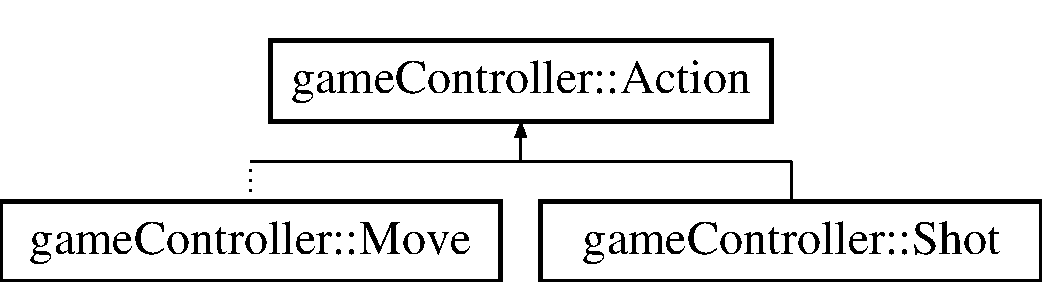
\includegraphics[height=2.000000cm]{classgame_controller_1_1_action}
\end{center}
\end{figure}
\subsection*{Public Member Functions}
\begin{DoxyCompactItemize}
\item 
\hyperlink{classgame_controller_1_1_action_a2bd3423680c850dcb88aa860a84cddee}{Action} ()=default
\item 
\hyperlink{classgame_controller_1_1_action_a74a9ef91e17f72be6d8f521931f24437}{Action} (std\-::shared\-\_\-ptr$<$ \hyperlink{classgame_model_1_1_environment}{game\-Model\-::\-Environment} $>$ env, std\-::shared\-\_\-ptr$<$ \hyperlink{classgame_model_1_1_player}{game\-Model\-::\-Player} $>$ actor, \hyperlink{structgame_model_1_1_position}{game\-Model\-::\-Position} target)
\item 
\hypertarget{classgame_controller_1_1_action_a7243ec6fcf8a36506d1a35a4abe333ec}{virtual auto {\bfseries execute} () const -\/$>$ std\-::pair$<$ std\-::vector$<$ Shot\-Result $>$, std\-::vector$<$ game\-Model\-::\-Foul $>$$>$=0}\label{classgame_controller_1_1_action_a7243ec6fcf8a36506d1a35a4abe333ec}

\item 
\hypertarget{classgame_controller_1_1_action_a9d9a301180bd5cd54a12ec912daf35c1}{virtual auto {\bfseries success\-Prob} () const -\/$>$ double=0}\label{classgame_controller_1_1_action_a9d9a301180bd5cd54a12ec912daf35c1}

\item 
\hypertarget{classgame_controller_1_1_action_abd249c0f371aac9d98a4fa60c4fd94c1}{virtual auto {\bfseries check} () const -\/$>$ Action\-Check\-Result=0}\label{classgame_controller_1_1_action_abd249c0f371aac9d98a4fa60c4fd94c1}

\item 
\hypertarget{classgame_controller_1_1_action_acb7adedb0d67ce14e3d825567dbc8585}{virtual auto {\bfseries execute\-All} () const -\/$>$ std\-::vector$<$ std\-::pair$<$ \hyperlink{classgame_model_1_1_environment}{game\-Model\-::\-Environment}, double $>$$>$=0}\label{classgame_controller_1_1_action_acb7adedb0d67ce14e3d825567dbc8585}

\end{DoxyCompactItemize}
\subsection*{Protected Attributes}
\begin{DoxyCompactItemize}
\item 
\hypertarget{classgame_controller_1_1_action_a3941f4d176b7631affa1710990a0cb0f}{std\-::shared\-\_\-ptr\\*
$<$ \hyperlink{classgame_model_1_1_player}{game\-Model\-::\-Player} $>$ {\bfseries actor}}\label{classgame_controller_1_1_action_a3941f4d176b7631affa1710990a0cb0f}

\item 
\hypertarget{classgame_controller_1_1_action_a77683804e62e608d15e4cc311c278c48}{std\-::shared\-\_\-ptr\\*
$<$ \hyperlink{classgame_model_1_1_environment}{game\-Model\-::\-Environment} $>$ {\bfseries env}}\label{classgame_controller_1_1_action_a77683804e62e608d15e4cc311c278c48}

\item 
\hypertarget{classgame_controller_1_1_action_a84d08ebf577d3ef17ae996c4394d61b6}{\hyperlink{structgame_model_1_1_position}{game\-Model\-::\-Position} {\bfseries target} \{\}}\label{classgame_controller_1_1_action_a84d08ebf577d3ef17ae996c4394d61b6}

\end{DoxyCompactItemize}


\subsection{Constructor \& Destructor Documentation}
\hypertarget{classgame_controller_1_1_action_a2bd3423680c850dcb88aa860a84cddee}{\index{game\-Controller\-::\-Action@{game\-Controller\-::\-Action}!Action@{Action}}
\index{Action@{Action}!gameController::Action@{game\-Controller\-::\-Action}}
\subsubsection[{Action}]{\setlength{\rightskip}{0pt plus 5cm}game\-Controller\-::\-Action\-::\-Action (
\begin{DoxyParamCaption}
{}
\end{DoxyParamCaption}
)\hspace{0.3cm}{\ttfamily [default]}}}\label{classgame_controller_1_1_action_a2bd3423680c850dcb88aa860a84cddee}
default constructor for the \hyperlink{classgame_controller_1_1_action}{Action} class. \hypertarget{classgame_controller_1_1_action_a74a9ef91e17f72be6d8f521931f24437}{\index{game\-Controller\-::\-Action@{game\-Controller\-::\-Action}!Action@{Action}}
\index{Action@{Action}!gameController::Action@{game\-Controller\-::\-Action}}
\subsubsection[{Action}]{\setlength{\rightskip}{0pt plus 5cm}game\-Controller\-::\-Action\-::\-Action (
\begin{DoxyParamCaption}
\item[{std\-::shared\-\_\-ptr$<$ {\bf game\-Model\-::\-Environment} $>$}]{env, }
\item[{std\-::shared\-\_\-ptr$<$ {\bf game\-Model\-::\-Player} $>$}]{actor, }
\item[{{\bf game\-Model\-::\-Position}}]{target}
\end{DoxyParamCaption}
)}}\label{classgame_controller_1_1_action_a74a9ef91e17f72be6d8f521931f24437}
main constructor for the \hyperlink{classgame_controller_1_1_action}{Action} class. 
\begin{DoxyParams}{Parameters}
{\em env} & The environment to operate on \\
\hline
{\em actor} & the actor \\
\hline
{\em target} & the target position \\
\hline
\end{DoxyParams}


The documentation for this class was generated from the following files\-:\begin{DoxyCompactItemize}
\item 
/home/travis/build/\-So\-Pra-\/\-Team-\/10/\-Game\-Logic/Action.\-h\item 
/home/travis/build/\-So\-Pra-\/\-Team-\/10/\-Game\-Logic/Action.\-cpp\end{DoxyCompactItemize}

\hypertarget{classgame_model_1_1_ball}{\section{game\-Model\-:\-:Ball Class Reference}
\label{classgame_model_1_1_ball}\index{game\-Model\-::\-Ball@{game\-Model\-::\-Ball}}
}


{\ttfamily \#include $<$Game\-Model.\-h$>$}

Inheritance diagram for game\-Model\-:\-:Ball\-:\begin{figure}[H]
\begin{center}
\leavevmode
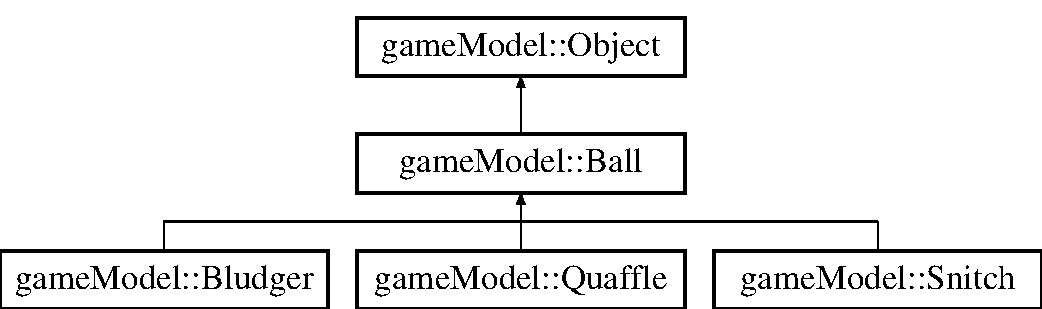
\includegraphics[height=3.000000cm]{classgame_model_1_1_ball}
\end{center}
\end{figure}
\subsection*{Public Member Functions}
\begin{DoxyCompactItemize}
\item 
\hypertarget{classgame_model_1_1_ball_a9f5a9659a7db01cdd3f4855309c40429}{{\bfseries Ball} (\hyperlink{structgame_model_1_1_position}{Position} position, communication\-::messages\-::types\-::\-Entity\-Id id)}\label{classgame_model_1_1_ball_a9f5a9659a7db01cdd3f4855309c40429}

\end{DoxyCompactItemize}
\subsection*{Additional Inherited Members}


\subsection{Detailed Description}
Represents non playable ball-\/objects 

The documentation for this class was generated from the following files\-:\begin{DoxyCompactItemize}
\item 
/home/travis/build/\-So\-Pra-\/\-Team-\/10/\-Game\-Logic/Game\-Model.\-h\item 
/home/travis/build/\-So\-Pra-\/\-Team-\/10/\-Game\-Logic/Game\-Model.\-cpp\end{DoxyCompactItemize}

\hypertarget{classgame_model_1_1_beater}{\section{game\-Model\-:\-:Beater Class Reference}
\label{classgame_model_1_1_beater}\index{game\-Model\-::\-Beater@{game\-Model\-::\-Beater}}
}
Inheritance diagram for game\-Model\-:\-:Beater\-:\begin{figure}[H]
\begin{center}
\leavevmode
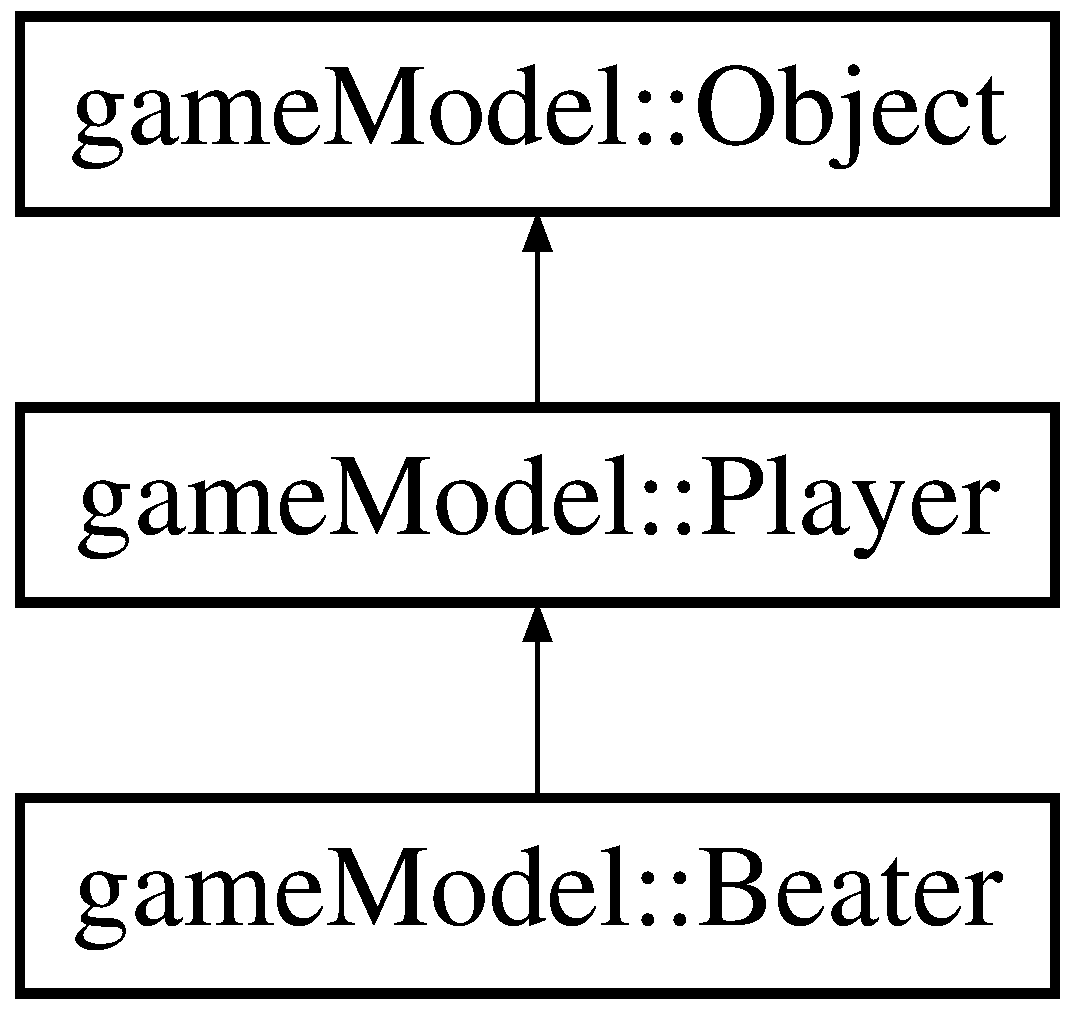
\includegraphics[height=3.000000cm]{classgame_model_1_1_beater}
\end{center}
\end{figure}
\subsection*{Public Member Functions}
\begin{DoxyCompactItemize}
\item 
\hypertarget{classgame_model_1_1_beater_ae2b91b72f61e55459889a89e1c5ebdac}{{\bfseries Beater} (\hyperlink{structgame_model_1_1_position}{Position} position, std\-::string name, communication\-::messages\-::types\-::\-Sex gender, communication\-::messages\-::types\-::\-Broom broom, communication\-::messages\-::types\-::\-Entity\-Id id)}\label{classgame_model_1_1_beater_ae2b91b72f61e55459889a89e1c5ebdac}

\end{DoxyCompactItemize}
\subsection*{Additional Inherited Members}


The documentation for this class was generated from the following file\-:\begin{DoxyCompactItemize}
\item 
/home/travis/build/\-So\-Pra-\/\-Team-\/10/\-Game\-Logic/Game\-Model.\-h\end{DoxyCompactItemize}

\hypertarget{classgame_model_1_1_bludger}{\section{game\-Model\-:\-:Bludger Class Reference}
\label{classgame_model_1_1_bludger}\index{game\-Model\-::\-Bludger@{game\-Model\-::\-Bludger}}
}
Inheritance diagram for game\-Model\-:\-:Bludger\-:\begin{figure}[H]
\begin{center}
\leavevmode
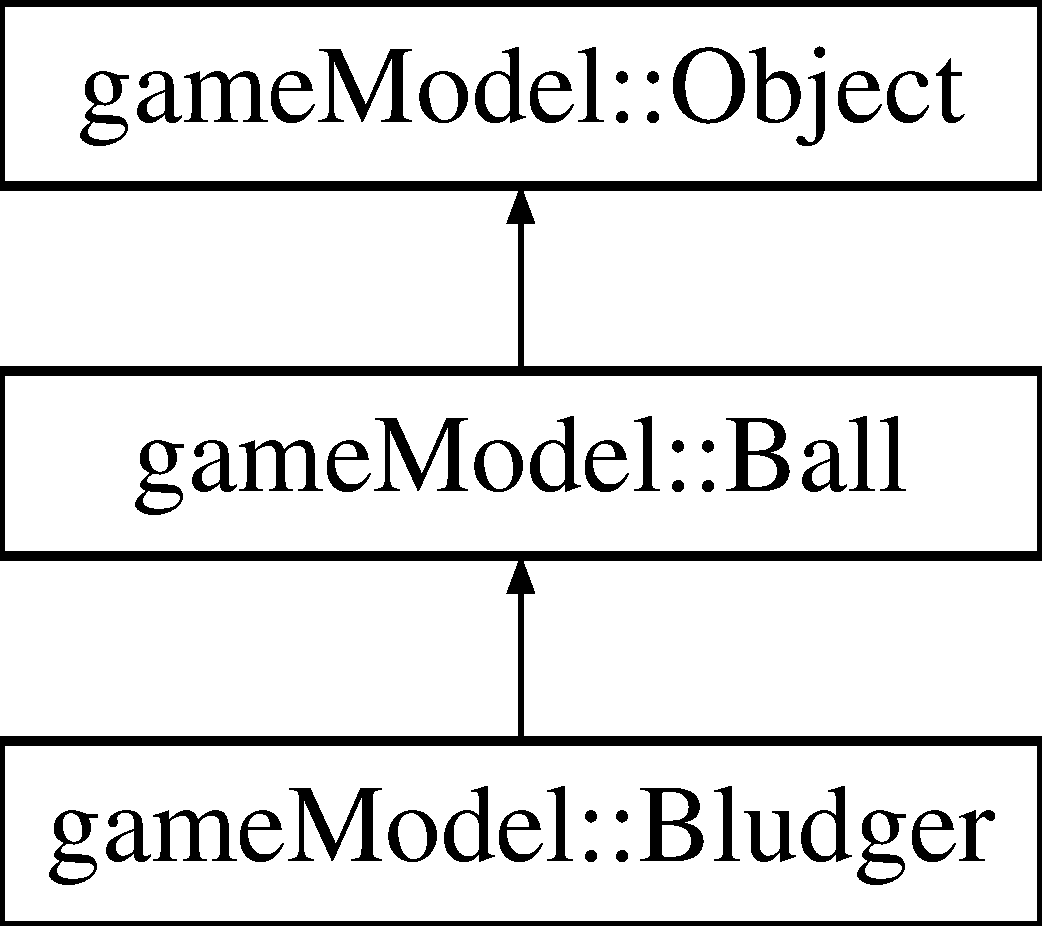
\includegraphics[height=3.000000cm]{classgame_model_1_1_bludger}
\end{center}
\end{figure}
\subsection*{Public Member Functions}
\begin{DoxyCompactItemize}
\item 
\hyperlink{classgame_model_1_1_bludger_a390de480fc712d0df7fe55ecc0fcff4d}{Bludger} (communication\-::messages\-::types\-::\-Entity\-Id id)
\item 
\hypertarget{classgame_model_1_1_bludger_a107364eb5e4d7d752483ad132c4a5eaa}{{\bfseries Bludger} (\hyperlink{structgame_model_1_1_position}{Position} position, communication\-::messages\-::types\-::\-Entity\-Id id)}\label{classgame_model_1_1_bludger_a107364eb5e4d7d752483ad132c4a5eaa}

\end{DoxyCompactItemize}
\subsection*{Additional Inherited Members}


\subsection{Constructor \& Destructor Documentation}
\hypertarget{classgame_model_1_1_bludger_a390de480fc712d0df7fe55ecc0fcff4d}{\index{game\-Model\-::\-Bludger@{game\-Model\-::\-Bludger}!Bludger@{Bludger}}
\index{Bludger@{Bludger}!gameModel::Bludger@{game\-Model\-::\-Bludger}}
\subsubsection[{Bludger}]{\setlength{\rightskip}{0pt plus 5cm}game\-Model\-::\-Bludger\-::\-Bludger (
\begin{DoxyParamCaption}
\item[{communication\-::messages\-::types\-::\-Entity\-Id}]{id}
\end{DoxyParamCaption}
)}}\label{classgame_model_1_1_bludger_a390de480fc712d0df7fe55ecc0fcff4d}
Places \hyperlink{classgame_model_1_1_bludger}{Bludger} in the centre of the field 

The documentation for this class was generated from the following files\-:\begin{DoxyCompactItemize}
\item 
/home/travis/build/\-So\-Pra-\/\-Team-\/10/\-Game\-Logic/Game\-Model.\-h\item 
/home/travis/build/\-So\-Pra-\/\-Team-\/10/\-Game\-Logic/Game\-Model.\-cpp\end{DoxyCompactItemize}

\hypertarget{classgame_model_1_1_chaser}{\section{game\-Model\-:\-:Chaser Class Reference}
\label{classgame_model_1_1_chaser}\index{game\-Model\-::\-Chaser@{game\-Model\-::\-Chaser}}
}
Inheritance diagram for game\-Model\-:\-:Chaser\-:\begin{figure}[H]
\begin{center}
\leavevmode
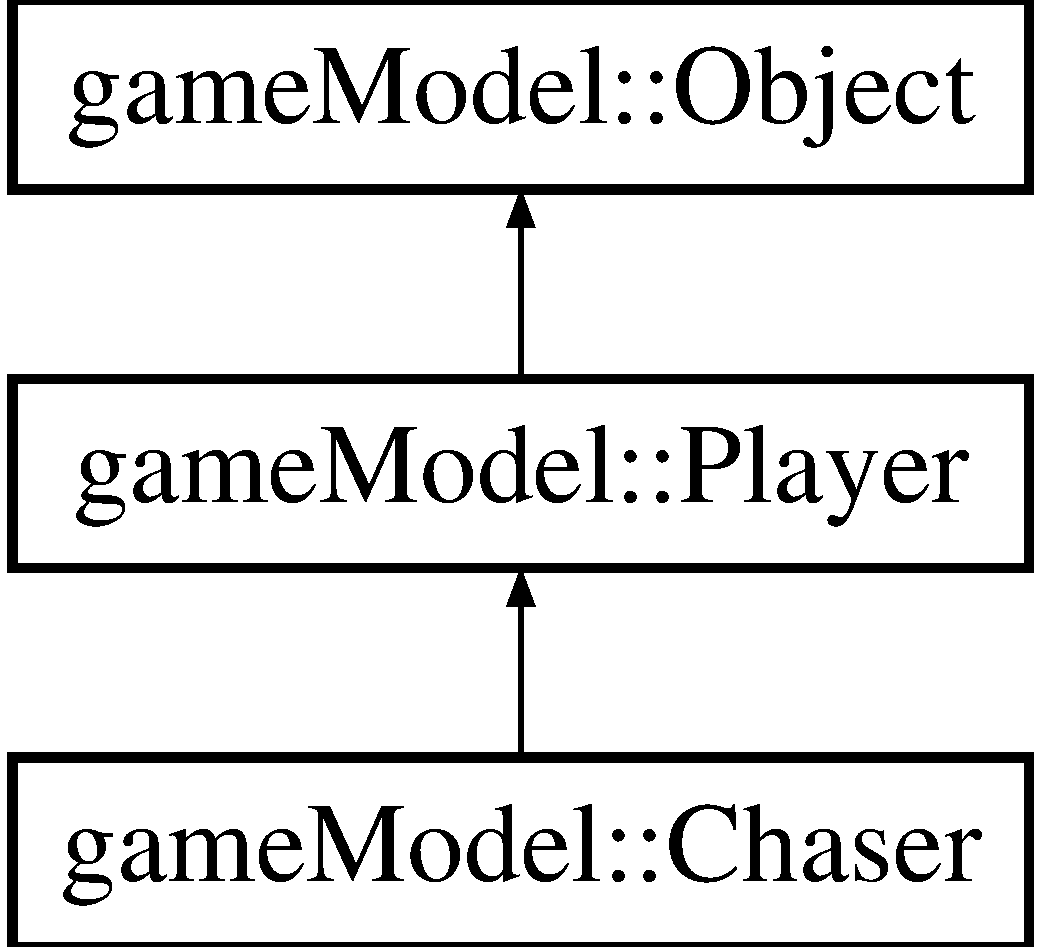
\includegraphics[height=3.000000cm]{classgame_model_1_1_chaser}
\end{center}
\end{figure}
\subsection*{Public Member Functions}
\begin{DoxyCompactItemize}
\item 
\hypertarget{classgame_model_1_1_chaser_a08d2698697ec6327798591f2e095389c}{{\bfseries Chaser} (\hyperlink{structgame_model_1_1_position}{Position} position, std\-::string name, communication\-::messages\-::types\-::\-Sex gender, communication\-::messages\-::types\-::\-Broom broom, communication\-::messages\-::types\-::\-Entity\-Id id)}\label{classgame_model_1_1_chaser_a08d2698697ec6327798591f2e095389c}

\end{DoxyCompactItemize}
\subsection*{Additional Inherited Members}


The documentation for this class was generated from the following file\-:\begin{DoxyCompactItemize}
\item 
/home/travis/build/\-So\-Pra-\/\-Team-\/10/\-Game\-Logic/Game\-Model.\-h\end{DoxyCompactItemize}

\hypertarget{classgame_model_1_1_config}{\section{game\-Model\-:\-:Config Class Reference}
\label{classgame_model_1_1_config}\index{game\-Model\-::\-Config@{game\-Model\-::\-Config}}
}


{\ttfamily \#include $<$Game\-Model.\-h$>$}

\subsection*{Public Member Functions}
\begin{DoxyCompactItemize}
\item 
\hypertarget{classgame_model_1_1_config_ad52aaf53a06d21ebedd5328f4190b8c1}{{\bfseries Config} (const communication\-::messages\-::broadcast\-::\-Match\-Config \&config)}\label{classgame_model_1_1_config_ad52aaf53a06d21ebedd5328f4190b8c1}

\item 
\hypertarget{classgame_model_1_1_config_a74534bffc047f6038453997965f75199}{{\bfseries Config} (unsigned int max\-Rounds, const \hyperlink{structgame_model_1_1_timeouts}{Timeouts} \&timeouts, const \hyperlink{structgame_model_1_1_foul_detection_probs}{Foul\-Detection\-Probs} \&foul\-Detection\-Probs, const \hyperlink{structgame_model_1_1_game_dynamics_probs}{Game\-Dynamics\-Probs} \&game\-Dynamics\-Probs, std\-::map$<$ communication\-::messages\-::types\-::\-Broom, double $>$ extra\-Turn\-Probs)}\label{classgame_model_1_1_config_a74534bffc047f6038453997965f75199}

\item 
double \hyperlink{classgame_model_1_1_config_a7e2134a72f3b75c43610d337abf8e9c0}{get\-Extra\-Turn\-Prob} (communication\-::messages\-::types\-::\-Broom broom) const 
\end{DoxyCompactItemize}
\subsection*{Data Fields}
\begin{DoxyCompactItemize}
\item 
\hypertarget{classgame_model_1_1_config_a9690fb78b42fcb9310d55d89fb49079e}{const unsigned int {\bfseries max\-Rounds}}\label{classgame_model_1_1_config_a9690fb78b42fcb9310d55d89fb49079e}

\item 
\hypertarget{classgame_model_1_1_config_a5757760f64e95fdc55489414e5e6d52e}{const \hyperlink{structgame_model_1_1_timeouts}{Timeouts} {\bfseries timeouts}}\label{classgame_model_1_1_config_a5757760f64e95fdc55489414e5e6d52e}

\item 
\hypertarget{classgame_model_1_1_config_a810141306fe0e5f8d3c445fed3c898a5}{const \hyperlink{structgame_model_1_1_foul_detection_probs}{Foul\-Detection\-Probs} {\bfseries foul\-Detection\-Probs}}\label{classgame_model_1_1_config_a810141306fe0e5f8d3c445fed3c898a5}

\item 
\hypertarget{classgame_model_1_1_config_ad88e428a62281ff69051f424bd4966c2}{const \hyperlink{structgame_model_1_1_game_dynamics_probs}{Game\-Dynamics\-Probs} {\bfseries game\-Dynamics\-Probs}}\label{classgame_model_1_1_config_ad88e428a62281ff69051f424bd4966c2}

\end{DoxyCompactItemize}


\subsection{Detailed Description}
Class containing metadata for a match 

\subsection{Member Function Documentation}
\hypertarget{classgame_model_1_1_config_a7e2134a72f3b75c43610d337abf8e9c0}{\index{game\-Model\-::\-Config@{game\-Model\-::\-Config}!get\-Extra\-Turn\-Prob@{get\-Extra\-Turn\-Prob}}
\index{get\-Extra\-Turn\-Prob@{get\-Extra\-Turn\-Prob}!gameModel::Config@{game\-Model\-::\-Config}}
\subsubsection[{get\-Extra\-Turn\-Prob}]{\setlength{\rightskip}{0pt plus 5cm}double game\-Model\-::\-Config\-::get\-Extra\-Turn\-Prob (
\begin{DoxyParamCaption}
\item[{communication\-::messages\-::types\-::\-Broom}]{broom}
\end{DoxyParamCaption}
) const}}\label{classgame_model_1_1_config_a7e2134a72f3b75c43610d337abf8e9c0}
Gets the probability of an extra turn with the specified Broom type 
\begin{DoxyParams}{Parameters}
{\em broom} & \\
\hline
\end{DoxyParams}
\begin{DoxyReturn}{Returns}

\end{DoxyReturn}


The documentation for this class was generated from the following files\-:\begin{DoxyCompactItemize}
\item 
/home/travis/build/\-So\-Pra-\/\-Team-\/10/\-Game\-Logic/Game\-Model.\-h\item 
/home/travis/build/\-So\-Pra-\/\-Team-\/10/\-Game\-Logic/Game\-Model.\-cpp\end{DoxyCompactItemize}

\hypertarget{classgame_model_1_1_environment}{\section{game\-Model\-:\-:Environment Class Reference}
\label{classgame_model_1_1_environment}\index{game\-Model\-::\-Environment@{game\-Model\-::\-Environment}}
}


{\ttfamily \#include $<$Game\-Model.\-h$>$}

\subsection*{Public Member Functions}
\begin{DoxyCompactItemize}
\item 
\hyperlink{classgame_model_1_1_environment_adbd10b9cd7a613334d51a4fa8536bdc0}{Environment} (communication\-::messages\-::broadcast\-::\-Match\-Config match\-Config, const communication\-::messages\-::request\-::\-Team\-Config \&team\-Config1, const communication\-::messages\-::request\-::\-Team\-Config \&team\-Config2, communication\-::messages\-::request\-::\-Team\-Formation team\-Formation1, communication\-::messages\-::request\-::\-Team\-Formation team\-Formation2)
\item 
\hyperlink{classgame_model_1_1_environment_a0b0292d09728665fce5cd2e175968c20}{Environment} (\hyperlink{classgame_model_1_1_config}{Config} config, std\-::shared\-\_\-ptr$<$ \hyperlink{classgame_model_1_1_team}{Team} $>$ team1, std\-::shared\-\_\-ptr$<$ \hyperlink{classgame_model_1_1_team}{Team} $>$ team2)
\item 
\hypertarget{classgame_model_1_1_environment_a3252830b5b67df1ed22a766660d76e4f}{{\bfseries Environment} (\hyperlink{classgame_model_1_1_config}{Config} config, std\-::shared\-\_\-ptr$<$ \hyperlink{classgame_model_1_1_team}{Team} $>$ team1, std\-::shared\-\_\-ptr$<$ \hyperlink{classgame_model_1_1_team}{Team} $>$ team2, std\-::shared\-\_\-ptr$<$ \hyperlink{classgame_model_1_1_quaffle}{Quaffle} $>$ quaffle, std\-::shared\-\_\-ptr$<$ \hyperlink{classgame_model_1_1_snitch}{Snitch} $>$ snitch, std\-::array$<$ std\-::shared\-\_\-ptr$<$ \hyperlink{classgame_model_1_1_bludger}{Bludger} $>$, 2 $>$ bludgers)}\label{classgame_model_1_1_environment_a3252830b5b67df1ed22a766660d76e4f}

\item 
auto \hyperlink{classgame_model_1_1_environment_a0c6939ea74a7dd670e5936b90d48dc65}{are\-Player\-In\-Same\-Team} (const std\-::shared\-\_\-ptr$<$ \hyperlink{classgame_model_1_1_player}{Player} $>$ \&p1, const std\-::shared\-\_\-ptr$<$ \hyperlink{classgame_model_1_1_player}{Player} $>$ \&p2) const -\/$>$ bool
\item 
auto \hyperlink{classgame_model_1_1_environment_a846741d971c9b1d21ad1ba2bd88532f1}{is\-Player\-In\-Own\-Restricted\-Zone} (const std\-::shared\-\_\-ptr$<$ \hyperlink{classgame_model_1_1_player}{Player} $>$ \&player) const -\/$>$ bool
\item 
auto \hyperlink{classgame_model_1_1_environment_a92637ac80e4dae2392a296bae5606b89}{is\-Player\-In\-Opponent\-Restricted\-Zone} (const std\-::shared\-\_\-ptr$<$ \hyperlink{classgame_model_1_1_player}{Player} $>$ \&player) const -\/$>$ bool
\item 
auto \hyperlink{classgame_model_1_1_environment_a33e0d834f58e41ad5551a06ee220076a}{get\-All\-Players} () const -\/$>$ std\-::array$<$ std\-::shared\-\_\-ptr$<$ \hyperlink{classgame_model_1_1_player}{Player} $>$, 14 $>$
\item 
auto \hyperlink{classgame_model_1_1_environment_a3122c0963d935543e2a7da1303772124}{get\-Team\-Mates} (const std\-::shared\-\_\-ptr$<$ \hyperlink{classgame_model_1_1_player}{Player} $>$ \&player) const -\/$>$ std\-::array$<$ std\-::shared\-\_\-ptr$<$ \hyperlink{classgame_model_1_1_player}{Player} $>$, 6 $>$
\item 
auto \hyperlink{classgame_model_1_1_environment_ab3bc9e490d18df58fbbe4f5f3dfd1b05}{get\-Opponents} (const std\-::shared\-\_\-ptr$<$ \hyperlink{classgame_model_1_1_player}{Player} $>$ \&player) const -\/$>$ std\-::array$<$ std\-::shared\-\_\-ptr$<$ \hyperlink{classgame_model_1_1_player}{Player} $>$, 7 $>$
\item 
bool \hyperlink{classgame_model_1_1_environment_a1e3c326a8a358e9de0e5144ac5a42af2}{cell\-Is\-Free} (const \hyperlink{structgame_model_1_1_position}{Position} \&position) const 
\item 
auto \hyperlink{classgame_model_1_1_environment_a9ce8f0bc1d424b585bdc030205d48903}{get\-All\-Player\-Free\-Cells\-Around} (const \hyperlink{structgame_model_1_1_position}{Position} \&position) const -\/$>$ std\-::vector$<$ \hyperlink{structgame_model_1_1_position}{Position} $>$
\item 
auto \hyperlink{classgame_model_1_1_environment_ad50b8cb84c76a6dbbfa9f8210918a4c2}{get\-Player} (const \hyperlink{structgame_model_1_1_position}{Position} \&position) const -\/$>$ std\-::optional$<$ std\-::shared\-\_\-ptr$<$ \hyperlink{classgame_model_1_1_player}{Player} $>$$>$
\item 
auto \hyperlink{classgame_model_1_1_environment_a4d07c3194e35ffc1295a81c43c616540}{get\-Player\-By\-Id} (communication\-::messages\-::types\-::\-Entity\-Id id) const -\/$>$ std\-::shared\-\_\-ptr$<$ \hyperlink{classgame_model_1_1_player}{Player} $>$
\item 
auto \hyperlink{classgame_model_1_1_environment_a393a4957114c2361f17bc84d00cec55f}{get\-Team} (const std\-::shared\-\_\-ptr$<$ \hyperlink{classgame_model_1_1_player}{Player} $>$ \&player) const -\/$>$ std\-::shared\-\_\-ptr$<$ \hyperlink{classgame_model_1_1_team}{Team} $>$
\item 
auto \hyperlink{classgame_model_1_1_environment_a6dc6b12234cb9d31841b5d23153cb22d}{get\-All\-Free\-Cells} () -\/$>$ std\-::array$<$ \hyperlink{structgame_model_1_1_position}{Position}, 179 $>$
\item 
void \hyperlink{classgame_model_1_1_environment_a585e52dc36311ec40c350cb2a7fae9c3}{place\-Player\-On\-Random\-Free\-Cell} (const std\-::shared\-\_\-ptr$<$ \hyperlink{classgame_model_1_1_player}{Player} $>$ \&player)
\end{DoxyCompactItemize}
\subsection*{Static Public Member Functions}
\begin{DoxyCompactItemize}
\item 
static Cell \hyperlink{classgame_model_1_1_environment_a7c095b6202f82cc67d89aa3ec66f387d}{get\-Cell} (int x, int y)
\item 
static Cell \hyperlink{classgame_model_1_1_environment_a71dc1b8596a609a49215beb0d0870489}{get\-Cell} (const \hyperlink{structgame_model_1_1_position}{Position} \&position)
\item 
static auto \hyperlink{classgame_model_1_1_environment_a3eae4f5c6ac23d48c10a6688340b0ba9}{get\-Surrounding\-Positions} (const \hyperlink{structgame_model_1_1_position}{Position} \&position) -\/$>$ std\-::vector$<$ \hyperlink{structgame_model_1_1_position}{Position} $>$
\item 
\hypertarget{classgame_model_1_1_environment_a9718a31bd8e763a69a89028977d3dc5a}{static auto {\bfseries get\-Goals\-Left} () -\/$>$ std\-::array$<$ \hyperlink{structgame_model_1_1_position}{Position}, 3 $>$}\label{classgame_model_1_1_environment_a9718a31bd8e763a69a89028977d3dc5a}

\item 
\hypertarget{classgame_model_1_1_environment_a2614e33c697e1f433338a555b907186b}{static auto {\bfseries get\-Goals\-Right} () -\/$>$ std\-::array$<$ \hyperlink{structgame_model_1_1_position}{Position}, 3 $>$}\label{classgame_model_1_1_environment_a2614e33c697e1f433338a555b907186b}

\item 
static auto \hyperlink{classgame_model_1_1_environment_a13fbde88faea456678ae3471f20b11c2}{get\-All\-Valid\-Cells} () -\/$>$ std\-::array$<$ \hyperlink{structgame_model_1_1_position}{Position}, 193 $>$
\end{DoxyCompactItemize}
\subsection*{Data Fields}
\begin{DoxyCompactItemize}
\item 
\hypertarget{classgame_model_1_1_environment_ab279f79f3801407b32364c5561ba4dcf}{\hyperlink{classgame_model_1_1_config}{Config} {\bfseries config}}\label{classgame_model_1_1_environment_ab279f79f3801407b32364c5561ba4dcf}

\item 
\hypertarget{classgame_model_1_1_environment_a2e14ce1ffd7e2a129ae81c686adbef0f}{std\-::shared\-\_\-ptr$<$ \hyperlink{classgame_model_1_1_team}{Team} $>$ {\bfseries team1}}\label{classgame_model_1_1_environment_a2e14ce1ffd7e2a129ae81c686adbef0f}

\item 
\hypertarget{classgame_model_1_1_environment_a24a032c88b96f1aa9dc33cbacb5a85b7}{std\-::shared\-\_\-ptr$<$ \hyperlink{classgame_model_1_1_team}{Team} $>$ {\bfseries team2}}\label{classgame_model_1_1_environment_a24a032c88b96f1aa9dc33cbacb5a85b7}

\item 
\hypertarget{classgame_model_1_1_environment_a53045a75cb3c499bdfe45f2d3d36752f}{std\-::shared\-\_\-ptr$<$ \hyperlink{classgame_model_1_1_quaffle}{Quaffle} $>$ {\bfseries quaffle}}\label{classgame_model_1_1_environment_a53045a75cb3c499bdfe45f2d3d36752f}

\item 
\hypertarget{classgame_model_1_1_environment_aec8a2937f90f5ff967bbc57f17ffc15f}{std\-::shared\-\_\-ptr$<$ \hyperlink{classgame_model_1_1_snitch}{Snitch} $>$ {\bfseries snitch}}\label{classgame_model_1_1_environment_aec8a2937f90f5ff967bbc57f17ffc15f}

\item 
\hypertarget{classgame_model_1_1_environment_afe22e5667c13829e787ef4df6a9e9ee8}{std\-::array$<$ std\-::shared\-\_\-ptr\\*
$<$ \hyperlink{classgame_model_1_1_bludger}{Bludger} $>$, 2 $>$ {\bfseries bludgers}}\label{classgame_model_1_1_environment_afe22e5667c13829e787ef4df6a9e9ee8}

\end{DoxyCompactItemize}


\subsection{Detailed Description}
Represents a game state 

\subsection{Constructor \& Destructor Documentation}
\hypertarget{classgame_model_1_1_environment_adbd10b9cd7a613334d51a4fa8536bdc0}{\index{game\-Model\-::\-Environment@{game\-Model\-::\-Environment}!Environment@{Environment}}
\index{Environment@{Environment}!gameModel::Environment@{game\-Model\-::\-Environment}}
\subsubsection[{Environment}]{\setlength{\rightskip}{0pt plus 5cm}game\-Model\-::\-Environment\-::\-Environment (
\begin{DoxyParamCaption}
\item[{communication\-::messages\-::broadcast\-::\-Match\-Config}]{match\-Config, }
\item[{const communication\-::messages\-::request\-::\-Team\-Config \&}]{team\-Config1, }
\item[{const communication\-::messages\-::request\-::\-Team\-Config \&}]{team\-Config2, }
\item[{communication\-::messages\-::request\-::\-Team\-Formation}]{team\-Formation1, }
\item[{communication\-::messages\-::request\-::\-Team\-Formation}]{team\-Formation2}
\end{DoxyParamCaption}
)}}\label{classgame_model_1_1_environment_adbd10b9cd7a613334d51a4fa8536bdc0}
Constructs an \hyperlink{classgame_model_1_1_environment}{Environment} from server config types 
\begin{DoxyParams}{Parameters}
{\em match\-Config} & \\
\hline
{\em team\-Config} & \\
\hline
{\em team\-Formation} & \\
\hline
\end{DoxyParams}
\hypertarget{classgame_model_1_1_environment_a0b0292d09728665fce5cd2e175968c20}{\index{game\-Model\-::\-Environment@{game\-Model\-::\-Environment}!Environment@{Environment}}
\index{Environment@{Environment}!gameModel::Environment@{game\-Model\-::\-Environment}}
\subsubsection[{Environment}]{\setlength{\rightskip}{0pt plus 5cm}game\-Model\-::\-Environment\-::\-Environment (
\begin{DoxyParamCaption}
\item[{{\bf Config}}]{config, }
\item[{std\-::shared\-\_\-ptr$<$ {\bf Team} $>$}]{team1, }
\item[{std\-::shared\-\_\-ptr$<$ {\bf Team} $>$}]{team2}
\end{DoxyParamCaption}
)}}\label{classgame_model_1_1_environment_a0b0292d09728665fce5cd2e175968c20}
Automatically places all balls at the correct location 
\begin{DoxyParams}{Parameters}
{\em config} & \\
\hline
{\em team1} & \\
\hline
{\em team2} & \\
\hline
\end{DoxyParams}


\subsection{Member Function Documentation}
\hypertarget{classgame_model_1_1_environment_a0c6939ea74a7dd670e5936b90d48dc65}{\index{game\-Model\-::\-Environment@{game\-Model\-::\-Environment}!are\-Player\-In\-Same\-Team@{are\-Player\-In\-Same\-Team}}
\index{are\-Player\-In\-Same\-Team@{are\-Player\-In\-Same\-Team}!gameModel::Environment@{game\-Model\-::\-Environment}}
\subsubsection[{are\-Player\-In\-Same\-Team}]{\setlength{\rightskip}{0pt plus 5cm}auto game\-Model\-::\-Environment\-::are\-Player\-In\-Same\-Team (
\begin{DoxyParamCaption}
\item[{const std\-::shared\-\_\-ptr$<$ {\bf Player} $>$ \&}]{p1, }
\item[{const std\-::shared\-\_\-ptr$<$ {\bf Player} $>$ \&}]{p2}
\end{DoxyParamCaption}
) const -\/$>$ bool}}\label{classgame_model_1_1_environment_a0c6939ea74a7dd670e5936b90d48dc65}
tests if two players are in the same team. 
\begin{DoxyParams}{Parameters}
{\em p1} & player 1. \\
\hline
{\em p2} & player 2. \\
\hline
\end{DoxyParams}
\begin{DoxyReturn}{Returns}
if the players are in the same team true, else false. 
\end{DoxyReturn}
\hypertarget{classgame_model_1_1_environment_a1e3c326a8a358e9de0e5144ac5a42af2}{\index{game\-Model\-::\-Environment@{game\-Model\-::\-Environment}!cell\-Is\-Free@{cell\-Is\-Free}}
\index{cell\-Is\-Free@{cell\-Is\-Free}!gameModel::Environment@{game\-Model\-::\-Environment}}
\subsubsection[{cell\-Is\-Free}]{\setlength{\rightskip}{0pt plus 5cm}bool game\-Model\-::\-Environment\-::cell\-Is\-Free (
\begin{DoxyParamCaption}
\item[{const {\bf Position} \&}]{position}
\end{DoxyParamCaption}
) const}}\label{classgame_model_1_1_environment_a1e3c326a8a358e9de0e5144ac5a42af2}
Determines whether the given \hyperlink{structgame_model_1_1_position}{Position} is occupied by a \hyperlink{classgame_model_1_1_player}{Player} 
\begin{DoxyParams}{Parameters}
{\em position} & the position to be checked \\
\hline
\end{DoxyParams}
\begin{DoxyReturn}{Returns}
true if occupied, false otherwise 
\end{DoxyReturn}
\hypertarget{classgame_model_1_1_environment_a6dc6b12234cb9d31841b5d23153cb22d}{\index{game\-Model\-::\-Environment@{game\-Model\-::\-Environment}!get\-All\-Free\-Cells@{get\-All\-Free\-Cells}}
\index{get\-All\-Free\-Cells@{get\-All\-Free\-Cells}!gameModel::Environment@{game\-Model\-::\-Environment}}
\subsubsection[{get\-All\-Free\-Cells}]{\setlength{\rightskip}{0pt plus 5cm}auto game\-Model\-::\-Environment\-::get\-All\-Free\-Cells (
\begin{DoxyParamCaption}
{}
\end{DoxyParamCaption}
) -\/$>$ std\-::array$<${\bf Position}, 179$>$}}\label{classgame_model_1_1_environment_a6dc6b12234cb9d31841b5d23153cb22d}
Gets all valid cells not occupied by players \begin{DoxyReturn}{Returns}

\end{DoxyReturn}
\hypertarget{classgame_model_1_1_environment_a9ce8f0bc1d424b585bdc030205d48903}{\index{game\-Model\-::\-Environment@{game\-Model\-::\-Environment}!get\-All\-Player\-Free\-Cells\-Around@{get\-All\-Player\-Free\-Cells\-Around}}
\index{get\-All\-Player\-Free\-Cells\-Around@{get\-All\-Player\-Free\-Cells\-Around}!gameModel::Environment@{game\-Model\-::\-Environment}}
\subsubsection[{get\-All\-Player\-Free\-Cells\-Around}]{\setlength{\rightskip}{0pt plus 5cm}auto game\-Model\-::\-Environment\-::get\-All\-Player\-Free\-Cells\-Around (
\begin{DoxyParamCaption}
\item[{const {\bf Position} \&}]{position}
\end{DoxyParamCaption}
) const -\/$>$ std\-::vector$<${\bf Position}$>$}}\label{classgame_model_1_1_environment_a9ce8f0bc1d424b585bdc030205d48903}
get all Positions around a given position where no other player is on. If all surrounding cells are blocked the search window is enlarged until a free cell is found 
\begin{DoxyParams}{Parameters}
{\em position} & the position to be checked \\
\hline
\end{DoxyParams}
\begin{DoxyReturn}{Returns}

\end{DoxyReturn}
\hypertarget{classgame_model_1_1_environment_a33e0d834f58e41ad5551a06ee220076a}{\index{game\-Model\-::\-Environment@{game\-Model\-::\-Environment}!get\-All\-Players@{get\-All\-Players}}
\index{get\-All\-Players@{get\-All\-Players}!gameModel::Environment@{game\-Model\-::\-Environment}}
\subsubsection[{get\-All\-Players}]{\setlength{\rightskip}{0pt plus 5cm}auto game\-Model\-::\-Environment\-::get\-All\-Players (
\begin{DoxyParamCaption}
{}
\end{DoxyParamCaption}
) const -\/$>$ std\-::array$<$std\-::shared\-\_\-ptr$<${\bf Player}$>$, 14$>$}}\label{classgame_model_1_1_environment_a33e0d834f58e41ad5551a06ee220076a}
Gets all players on the field \begin{DoxyReturn}{Returns}

\end{DoxyReturn}
\hypertarget{classgame_model_1_1_environment_a13fbde88faea456678ae3471f20b11c2}{\index{game\-Model\-::\-Environment@{game\-Model\-::\-Environment}!get\-All\-Valid\-Cells@{get\-All\-Valid\-Cells}}
\index{get\-All\-Valid\-Cells@{get\-All\-Valid\-Cells}!gameModel::Environment@{game\-Model\-::\-Environment}}
\subsubsection[{get\-All\-Valid\-Cells}]{\setlength{\rightskip}{0pt plus 5cm}auto game\-Model\-::\-Environment\-::get\-All\-Valid\-Cells (
\begin{DoxyParamCaption}
{}
\end{DoxyParamCaption}
) -\/$>$ std\-::array$<${\bf Position}, 193$>$\hspace{0.3cm}{\ttfamily [static]}}}\label{classgame_model_1_1_environment_a13fbde88faea456678ae3471f20b11c2}
Gets all Positions which are not out of bounds \begin{DoxyReturn}{Returns}

\end{DoxyReturn}
\hypertarget{classgame_model_1_1_environment_a7c095b6202f82cc67d89aa3ec66f387d}{\index{game\-Model\-::\-Environment@{game\-Model\-::\-Environment}!get\-Cell@{get\-Cell}}
\index{get\-Cell@{get\-Cell}!gameModel::Environment@{game\-Model\-::\-Environment}}
\subsubsection[{get\-Cell}]{\setlength{\rightskip}{0pt plus 5cm}Cell game\-Model\-::\-Environment\-::get\-Cell (
\begin{DoxyParamCaption}
\item[{int}]{x, }
\item[{int}]{y}
\end{DoxyParamCaption}
)\hspace{0.3cm}{\ttfamily [static]}}}\label{classgame_model_1_1_environment_a7c095b6202f82cc67d89aa3ec66f387d}
Gets the type of the cell at position (x,y) 
\begin{DoxyParams}{Parameters}
{\em x} & x\-Position from left, 0 based \\
\hline
{\em y} & y\-Position from bottom, 0 based \\
\hline
\end{DoxyParams}
\begin{DoxyReturn}{Returns}
The corresponding Cell 
\end{DoxyReturn}
\hypertarget{classgame_model_1_1_environment_a71dc1b8596a609a49215beb0d0870489}{\index{game\-Model\-::\-Environment@{game\-Model\-::\-Environment}!get\-Cell@{get\-Cell}}
\index{get\-Cell@{get\-Cell}!gameModel::Environment@{game\-Model\-::\-Environment}}
\subsubsection[{get\-Cell}]{\setlength{\rightskip}{0pt plus 5cm}Cell game\-Model\-::\-Environment\-::get\-Cell (
\begin{DoxyParamCaption}
\item[{const {\bf Position} \&}]{position}
\end{DoxyParamCaption}
)\hspace{0.3cm}{\ttfamily [static]}}}\label{classgame_model_1_1_environment_a71dc1b8596a609a49215beb0d0870489}
See overloaded function above 
\begin{DoxyParams}{Parameters}
{\em position} & \\
\hline
\end{DoxyParams}
\begin{DoxyReturn}{Returns}

\end{DoxyReturn}
\hypertarget{classgame_model_1_1_environment_ab3bc9e490d18df58fbbe4f5f3dfd1b05}{\index{game\-Model\-::\-Environment@{game\-Model\-::\-Environment}!get\-Opponents@{get\-Opponents}}
\index{get\-Opponents@{get\-Opponents}!gameModel::Environment@{game\-Model\-::\-Environment}}
\subsubsection[{get\-Opponents}]{\setlength{\rightskip}{0pt plus 5cm}auto game\-Model\-::\-Environment\-::get\-Opponents (
\begin{DoxyParamCaption}
\item[{const std\-::shared\-\_\-ptr$<$ {\bf Player} $>$ \&}]{player}
\end{DoxyParamCaption}
) const -\/$>$ std\-::array$<$std\-::shared\-\_\-ptr$<${\bf Player}$>$, 7$>$}}\label{classgame_model_1_1_environment_ab3bc9e490d18df58fbbe4f5f3dfd1b05}
Gets all players from the opponent team of the given player 
\begin{DoxyParams}{Parameters}
{\em player} & \\
\hline
\end{DoxyParams}
\begin{DoxyReturn}{Returns}

\end{DoxyReturn}
\hypertarget{classgame_model_1_1_environment_ad50b8cb84c76a6dbbfa9f8210918a4c2}{\index{game\-Model\-::\-Environment@{game\-Model\-::\-Environment}!get\-Player@{get\-Player}}
\index{get\-Player@{get\-Player}!gameModel::Environment@{game\-Model\-::\-Environment}}
\subsubsection[{get\-Player}]{\setlength{\rightskip}{0pt plus 5cm}auto game\-Model\-::\-Environment\-::get\-Player (
\begin{DoxyParamCaption}
\item[{const {\bf Position} \&}]{position}
\end{DoxyParamCaption}
) const -\/$>$ std\-::optional$<$std\-::shared\-\_\-ptr$<${\bf Player}$>$$>$}}\label{classgame_model_1_1_environment_ad50b8cb84c76a6dbbfa9f8210918a4c2}
Returns player object at the specified position if one exists \begin{DoxyReturn}{Returns}

\end{DoxyReturn}
\hypertarget{classgame_model_1_1_environment_a4d07c3194e35ffc1295a81c43c616540}{\index{game\-Model\-::\-Environment@{game\-Model\-::\-Environment}!get\-Player\-By\-Id@{get\-Player\-By\-Id}}
\index{get\-Player\-By\-Id@{get\-Player\-By\-Id}!gameModel::Environment@{game\-Model\-::\-Environment}}
\subsubsection[{get\-Player\-By\-Id}]{\setlength{\rightskip}{0pt plus 5cm}auto game\-Model\-::\-Environment\-::get\-Player\-By\-Id (
\begin{DoxyParamCaption}
\item[{communication\-::messages\-::types\-::\-Entity\-Id}]{id}
\end{DoxyParamCaption}
) const -\/$>$ std\-::shared\-\_\-ptr$<${\bf Player}$>$}}\label{classgame_model_1_1_environment_a4d07c3194e35ffc1295a81c43c616540}
gets player by server entity id 
\begin{DoxyParams}{Parameters}
{\em id} & \\
\hline
\end{DoxyParams}

\begin{DoxyExceptions}{Exceptions}
{\em runtime\-\_\-error} & when player cannot be found \\
\hline
\end{DoxyExceptions}
\begin{DoxyReturn}{Returns}

\end{DoxyReturn}
\hypertarget{classgame_model_1_1_environment_a3eae4f5c6ac23d48c10a6688340b0ba9}{\index{game\-Model\-::\-Environment@{game\-Model\-::\-Environment}!get\-Surrounding\-Positions@{get\-Surrounding\-Positions}}
\index{get\-Surrounding\-Positions@{get\-Surrounding\-Positions}!gameModel::Environment@{game\-Model\-::\-Environment}}
\subsubsection[{get\-Surrounding\-Positions}]{\setlength{\rightskip}{0pt plus 5cm}auto game\-Model\-::\-Environment\-::get\-Surrounding\-Positions (
\begin{DoxyParamCaption}
\item[{const {\bf Position} \&}]{position}
\end{DoxyParamCaption}
) -\/$>$ std\-::vector$<${\bf Position}$>$\hspace{0.3cm}{\ttfamily [static]}}}\label{classgame_model_1_1_environment_a3eae4f5c6ac23d48c10a6688340b0ba9}
Gets all valid \hyperlink{structgame_model_1_1_position}{Position} surrounding the given position 
\begin{DoxyParams}{Parameters}
{\em position} & \\
\hline
\end{DoxyParams}
\begin{DoxyReturn}{Returns}

\end{DoxyReturn}
\hypertarget{classgame_model_1_1_environment_a393a4957114c2361f17bc84d00cec55f}{\index{game\-Model\-::\-Environment@{game\-Model\-::\-Environment}!get\-Team@{get\-Team}}
\index{get\-Team@{get\-Team}!gameModel::Environment@{game\-Model\-::\-Environment}}
\subsubsection[{get\-Team}]{\setlength{\rightskip}{0pt plus 5cm}auto game\-Model\-::\-Environment\-::get\-Team (
\begin{DoxyParamCaption}
\item[{const std\-::shared\-\_\-ptr$<$ {\bf Player} $>$ \&}]{player}
\end{DoxyParamCaption}
) const -\/$>$ std\-::shared\-\_\-ptr$<${\bf Team}$>$}}\label{classgame_model_1_1_environment_a393a4957114c2361f17bc84d00cec55f}
get the corresponding team of a player. 
\begin{DoxyParams}{Parameters}
{\em player} & the selected player. \\
\hline
\end{DoxyParams}
\begin{DoxyReturn}{Returns}
the team of a player. 
\end{DoxyReturn}
\hypertarget{classgame_model_1_1_environment_a3122c0963d935543e2a7da1303772124}{\index{game\-Model\-::\-Environment@{game\-Model\-::\-Environment}!get\-Team\-Mates@{get\-Team\-Mates}}
\index{get\-Team\-Mates@{get\-Team\-Mates}!gameModel::Environment@{game\-Model\-::\-Environment}}
\subsubsection[{get\-Team\-Mates}]{\setlength{\rightskip}{0pt plus 5cm}auto game\-Model\-::\-Environment\-::get\-Team\-Mates (
\begin{DoxyParamCaption}
\item[{const std\-::shared\-\_\-ptr$<$ {\bf Player} $>$ \&}]{player}
\end{DoxyParamCaption}
) const -\/$>$ std\-::array$<$std\-::shared\-\_\-ptr$<${\bf Player}$>$, 6$>$}}\label{classgame_model_1_1_environment_a3122c0963d935543e2a7da1303772124}
Gets all players in the same team as the given player, themselves excluded 
\begin{DoxyParams}{Parameters}
{\em player} & \\
\hline
\end{DoxyParams}
\begin{DoxyReturn}{Returns}

\end{DoxyReturn}
\hypertarget{classgame_model_1_1_environment_a92637ac80e4dae2392a296bae5606b89}{\index{game\-Model\-::\-Environment@{game\-Model\-::\-Environment}!is\-Player\-In\-Opponent\-Restricted\-Zone@{is\-Player\-In\-Opponent\-Restricted\-Zone}}
\index{is\-Player\-In\-Opponent\-Restricted\-Zone@{is\-Player\-In\-Opponent\-Restricted\-Zone}!gameModel::Environment@{game\-Model\-::\-Environment}}
\subsubsection[{is\-Player\-In\-Opponent\-Restricted\-Zone}]{\setlength{\rightskip}{0pt plus 5cm}auto game\-Model\-::\-Environment\-::is\-Player\-In\-Opponent\-Restricted\-Zone (
\begin{DoxyParamCaption}
\item[{const std\-::shared\-\_\-ptr$<$ {\bf Player} $>$ \&}]{player}
\end{DoxyParamCaption}
) const -\/$>$ bool}}\label{classgame_model_1_1_environment_a92637ac80e4dae2392a296bae5606b89}
checks if a player is in the opponent restricted zone. 
\begin{DoxyParams}{Parameters}
{\em player} & the player. \\
\hline
\end{DoxyParams}
\begin{DoxyReturn}{Returns}
true if player is in opponent restricted zone, else false; 
\end{DoxyReturn}
\hypertarget{classgame_model_1_1_environment_a846741d971c9b1d21ad1ba2bd88532f1}{\index{game\-Model\-::\-Environment@{game\-Model\-::\-Environment}!is\-Player\-In\-Own\-Restricted\-Zone@{is\-Player\-In\-Own\-Restricted\-Zone}}
\index{is\-Player\-In\-Own\-Restricted\-Zone@{is\-Player\-In\-Own\-Restricted\-Zone}!gameModel::Environment@{game\-Model\-::\-Environment}}
\subsubsection[{is\-Player\-In\-Own\-Restricted\-Zone}]{\setlength{\rightskip}{0pt plus 5cm}auto game\-Model\-::\-Environment\-::is\-Player\-In\-Own\-Restricted\-Zone (
\begin{DoxyParamCaption}
\item[{const std\-::shared\-\_\-ptr$<$ {\bf Player} $>$ \&}]{player}
\end{DoxyParamCaption}
) const -\/$>$ bool}}\label{classgame_model_1_1_environment_a846741d971c9b1d21ad1ba2bd88532f1}
checks if a player is in the own restricted zone. 
\begin{DoxyParams}{Parameters}
{\em player} & the player. \\
\hline
\end{DoxyParams}
\begin{DoxyReturn}{Returns}
true if player is in own restricted zone, else false; 
\end{DoxyReturn}
\hypertarget{classgame_model_1_1_environment_a585e52dc36311ec40c350cb2a7fae9c3}{\index{game\-Model\-::\-Environment@{game\-Model\-::\-Environment}!place\-Player\-On\-Random\-Free\-Cell@{place\-Player\-On\-Random\-Free\-Cell}}
\index{place\-Player\-On\-Random\-Free\-Cell@{place\-Player\-On\-Random\-Free\-Cell}!gameModel::Environment@{game\-Model\-::\-Environment}}
\subsubsection[{place\-Player\-On\-Random\-Free\-Cell}]{\setlength{\rightskip}{0pt plus 5cm}void game\-Model\-::\-Environment\-::place\-Player\-On\-Random\-Free\-Cell (
\begin{DoxyParamCaption}
\item[{const std\-::shared\-\_\-ptr$<$ {\bf Player} $>$ \&}]{player}
\end{DoxyParamCaption}
)}}\label{classgame_model_1_1_environment_a585e52dc36311ec40c350cb2a7fae9c3}
place a player on random free cell in his half of the game field. 
\begin{DoxyParams}{Parameters}
{\em player} & \\
\hline
\end{DoxyParams}


The documentation for this class was generated from the following files\-:\begin{DoxyCompactItemize}
\item 
/home/travis/build/\-So\-Pra-\/\-Team-\/10/\-Game\-Logic/Game\-Model.\-h\item 
/home/travis/build/\-So\-Pra-\/\-Team-\/10/\-Game\-Logic/Game\-Model.\-cpp\end{DoxyCompactItemize}

\hypertarget{classgame_model_1_1_fanblock}{\section{game\-Model\-:\-:Fanblock Class Reference}
\label{classgame_model_1_1_fanblock}\index{game\-Model\-::\-Fanblock@{game\-Model\-::\-Fanblock}}
}


{\ttfamily \#include $<$Game\-Model.\-h$>$}

\subsection*{Public Member Functions}
\begin{DoxyCompactItemize}
\item 
\hypertarget{classgame_model_1_1_fanblock_a31bb8f4e820a89c2de2d4edc7ba2ded7}{{\bfseries Fanblock} (int teleportation, int ranged\-Attack, int impulse, int snitch\-Push)}\label{classgame_model_1_1_fanblock_a31bb8f4e820a89c2de2d4edc7ba2ded7}

\item 
int \hyperlink{classgame_model_1_1_fanblock_a65c17009e532bcda8316a30d9e9433cd}{get\-Uses} (Interference\-Type fan) const 
\item 
void \hyperlink{classgame_model_1_1_fanblock_a1642d454e4547e75d63675a5f929314d}{ban\-Fan} (Interference\-Type fan)
\end{DoxyCompactItemize}


\subsection{Detailed Description}
Represents available fans for a \hyperlink{classgame_model_1_1_team}{Team} 

\subsection{Member Function Documentation}
\hypertarget{classgame_model_1_1_fanblock_a1642d454e4547e75d63675a5f929314d}{\index{game\-Model\-::\-Fanblock@{game\-Model\-::\-Fanblock}!ban\-Fan@{ban\-Fan}}
\index{ban\-Fan@{ban\-Fan}!gameModel::Fanblock@{game\-Model\-::\-Fanblock}}
\subsubsection[{ban\-Fan}]{\setlength{\rightskip}{0pt plus 5cm}void game\-Model\-::\-Fanblock\-::ban\-Fan (
\begin{DoxyParamCaption}
\item[{Interference\-Type}]{fan}
\end{DoxyParamCaption}
)}}\label{classgame_model_1_1_fanblock_a1642d454e4547e75d63675a5f929314d}
Bans a fan by decreasing the number of allowed uses by one 
\begin{DoxyParams}{Parameters}
{\em fan} & the fan to be banned \\
\hline
\end{DoxyParams}

\begin{DoxyExceptions}{Exceptions}
{\em std\-::invalid\-\_\-argument} & if there are no more fans left to ban of the given type \\
\hline
\end{DoxyExceptions}
\hypertarget{classgame_model_1_1_fanblock_a65c17009e532bcda8316a30d9e9433cd}{\index{game\-Model\-::\-Fanblock@{game\-Model\-::\-Fanblock}!get\-Uses@{get\-Uses}}
\index{get\-Uses@{get\-Uses}!gameModel::Fanblock@{game\-Model\-::\-Fanblock}}
\subsubsection[{get\-Uses}]{\setlength{\rightskip}{0pt plus 5cm}int game\-Model\-::\-Fanblock\-::get\-Uses (
\begin{DoxyParamCaption}
\item[{Interference\-Type}]{fan}
\end{DoxyParamCaption}
) const}}\label{classgame_model_1_1_fanblock_a65c17009e532bcda8316a30d9e9433cd}
gets the number of times the given fan might be used 
\begin{DoxyParams}{Parameters}
{\em fan} & the fan to check \\
\hline
\end{DoxyParams}
\begin{DoxyReturn}{Returns}
number of left uses 
\end{DoxyReturn}


The documentation for this class was generated from the following files\-:\begin{DoxyCompactItemize}
\item 
/home/travis/build/\-So\-Pra-\/\-Team-\/10/\-Game\-Logic/Game\-Model.\-h\item 
/home/travis/build/\-So\-Pra-\/\-Team-\/10/\-Game\-Logic/Game\-Model.\-cpp\end{DoxyCompactItemize}

\hypertarget{structgame_model_1_1_foul_detection_probs}{\section{game\-Model\-:\-:Foul\-Detection\-Probs Struct Reference}
\label{structgame_model_1_1_foul_detection_probs}\index{game\-Model\-::\-Foul\-Detection\-Probs@{game\-Model\-::\-Foul\-Detection\-Probs}}
}


{\ttfamily \#include $<$Game\-Model.\-h$>$}

\subsection*{Data Fields}
\begin{DoxyCompactItemize}
\item 
\hypertarget{structgame_model_1_1_foul_detection_probs_a4c83c08fe1e8b4f968aa6a7f7bd543bf}{double {\bfseries block\-Goal}}\label{structgame_model_1_1_foul_detection_probs_a4c83c08fe1e8b4f968aa6a7f7bd543bf}

\item 
\hypertarget{structgame_model_1_1_foul_detection_probs_add465246ba17e671a07231900449327f}{double {\bfseries charge\-Goal}}\label{structgame_model_1_1_foul_detection_probs_add465246ba17e671a07231900449327f}

\item 
\hypertarget{structgame_model_1_1_foul_detection_probs_ac9ca7891ddf324a2cd13d95f4402eabd}{double {\bfseries multiple\-Offence}}\label{structgame_model_1_1_foul_detection_probs_ac9ca7891ddf324a2cd13d95f4402eabd}

\item 
\hypertarget{structgame_model_1_1_foul_detection_probs_a7b9d645c139c65a0dd1f8241650a33b9}{double {\bfseries ramming}}\label{structgame_model_1_1_foul_detection_probs_a7b9d645c139c65a0dd1f8241650a33b9}

\item 
\hypertarget{structgame_model_1_1_foul_detection_probs_a3d2cf05df68174cc892fa14a62d2409c}{double {\bfseries block\-Snitch}}\label{structgame_model_1_1_foul_detection_probs_a3d2cf05df68174cc892fa14a62d2409c}

\item 
\hypertarget{structgame_model_1_1_foul_detection_probs_a357e0818580014857d179c4b4fd6868c}{double {\bfseries teleport}}\label{structgame_model_1_1_foul_detection_probs_a357e0818580014857d179c4b4fd6868c}

\item 
\hypertarget{structgame_model_1_1_foul_detection_probs_aa885ca6840d0692043d391b175c361a8}{double {\bfseries ranged\-Attack}}\label{structgame_model_1_1_foul_detection_probs_aa885ca6840d0692043d391b175c361a8}

\item 
\hypertarget{structgame_model_1_1_foul_detection_probs_a5bfd5f10ad171bf423a37776f0c2e7ed}{double {\bfseries impulse}}\label{structgame_model_1_1_foul_detection_probs_a5bfd5f10ad171bf423a37776f0c2e7ed}

\item 
\hypertarget{structgame_model_1_1_foul_detection_probs_ae3103298aff06049e468bc27d3946f3a}{double {\bfseries snitch\-Push}}\label{structgame_model_1_1_foul_detection_probs_ae3103298aff06049e468bc27d3946f3a}

\end{DoxyCompactItemize}


\subsection{Detailed Description}
Probabilities for detecting a foul 

The documentation for this struct was generated from the following file\-:\begin{DoxyCompactItemize}
\item 
/home/travis/build/\-So\-Pra-\/\-Team-\/10/\-Game\-Logic/Game\-Model.\-h\end{DoxyCompactItemize}

\hypertarget{structgame_model_1_1_game_dynamics_probs}{\section{game\-Model\-:\-:Game\-Dynamics\-Probs Struct Reference}
\label{structgame_model_1_1_game_dynamics_probs}\index{game\-Model\-::\-Game\-Dynamics\-Probs@{game\-Model\-::\-Game\-Dynamics\-Probs}}
}


{\ttfamily \#include $<$Game\-Model.\-h$>$}

\subsection*{Data Fields}
\begin{DoxyCompactItemize}
\item 
\hypertarget{structgame_model_1_1_game_dynamics_probs_a74398d5b822aad0c10e6e53882041884}{double {\bfseries throw\-Success}}\label{structgame_model_1_1_game_dynamics_probs_a74398d5b822aad0c10e6e53882041884}

\item 
\hypertarget{structgame_model_1_1_game_dynamics_probs_ab3e3fb13854097c6ddff28312a9aae52}{double {\bfseries knock\-Out}}\label{structgame_model_1_1_game_dynamics_probs_ab3e3fb13854097c6ddff28312a9aae52}

\item 
\hypertarget{structgame_model_1_1_game_dynamics_probs_ab270ff3325b31bc930ddcfa7b2dba937}{double {\bfseries fool\-Away}}\label{structgame_model_1_1_game_dynamics_probs_ab270ff3325b31bc930ddcfa7b2dba937}

\item 
\hypertarget{structgame_model_1_1_game_dynamics_probs_a48d76287b9322c815db5cce2e41149f5}{double {\bfseries catch\-Snitch}}\label{structgame_model_1_1_game_dynamics_probs_a48d76287b9322c815db5cce2e41149f5}

\item 
\hypertarget{structgame_model_1_1_game_dynamics_probs_a2e343d8ba7e8fe00b0802fa25a8eb1af}{double {\bfseries catch\-Quaffle}}\label{structgame_model_1_1_game_dynamics_probs_a2e343d8ba7e8fe00b0802fa25a8eb1af}

\item 
\hypertarget{structgame_model_1_1_game_dynamics_probs_a013c19aa13af71b274133592d00c4fad}{double {\bfseries wrest\-Quaffle}}\label{structgame_model_1_1_game_dynamics_probs_a013c19aa13af71b274133592d00c4fad}

\end{DoxyCompactItemize}


\subsection{Detailed Description}
Probabilities for standard gameplay 

The documentation for this struct was generated from the following file\-:\begin{DoxyCompactItemize}
\item 
/home/travis/build/\-So\-Pra-\/\-Team-\/10/\-Game\-Logic/Game\-Model.\-h\end{DoxyCompactItemize}

\hypertarget{classgame_controller_1_1_impulse}{\section{game\-Controller\-:\-:Impulse Class Reference}
\label{classgame_controller_1_1_impulse}\index{game\-Controller\-::\-Impulse@{game\-Controller\-::\-Impulse}}
}
Inheritance diagram for game\-Controller\-:\-:Impulse\-:\begin{figure}[H]
\begin{center}
\leavevmode
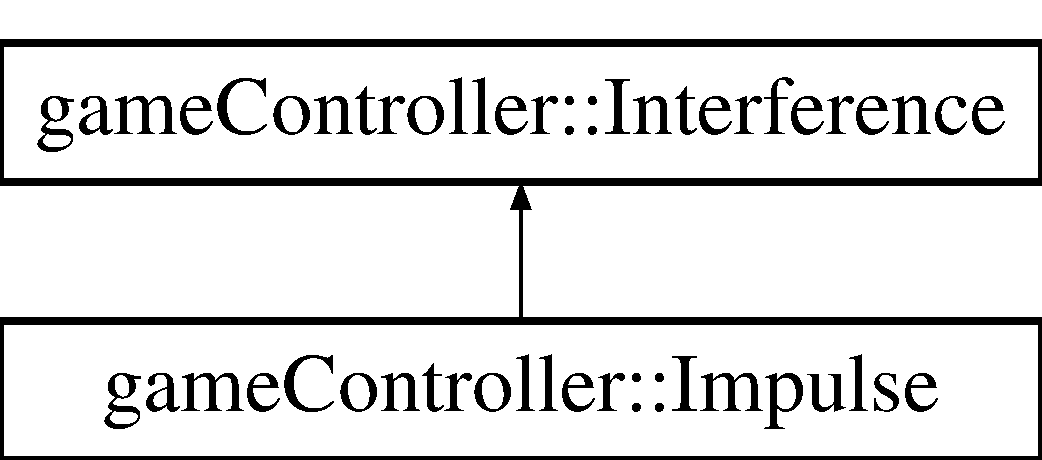
\includegraphics[height=2.000000cm]{classgame_controller_1_1_impulse}
\end{center}
\end{figure}
\subsection*{Public Member Functions}
\begin{DoxyCompactItemize}
\item 
\hypertarget{classgame_controller_1_1_impulse_a37354f13fe1dfb38e78b59f606961ad6}{{\bfseries Impulse} (std\-::shared\-\_\-ptr$<$ \hyperlink{classgame_model_1_1_environment}{game\-Model\-::\-Environment} $>$ env, std\-::shared\-\_\-ptr$<$ \hyperlink{classgame_model_1_1_team}{game\-Model\-::\-Team} $>$ team)}\label{classgame_controller_1_1_impulse_a37354f13fe1dfb38e78b59f606961ad6}

\item 
void \hyperlink{classgame_controller_1_1_impulse_aec92c13c5a3a55da3f8d948354a9b4f4}{execute} () const override
\end{DoxyCompactItemize}
\subsection*{Additional Inherited Members}


\subsection{Member Function Documentation}
\hypertarget{classgame_controller_1_1_impulse_aec92c13c5a3a55da3f8d948354a9b4f4}{\index{game\-Controller\-::\-Impulse@{game\-Controller\-::\-Impulse}!execute@{execute}}
\index{execute@{execute}!gameController::Impulse@{game\-Controller\-::\-Impulse}}
\subsubsection[{execute}]{\setlength{\rightskip}{0pt plus 5cm}void game\-Controller\-::\-Impulse\-::execute (
\begin{DoxyParamCaption}
{}
\end{DoxyParamCaption}
) const\hspace{0.3cm}{\ttfamily [override]}, {\ttfamily [virtual]}}}\label{classgame_controller_1_1_impulse_aec92c13c5a3a55da3f8d948354a9b4f4}
If a Keeper or Chaser holds the quaffle, quaffle is moved to a random free adjacent position 

Implements \hyperlink{classgame_controller_1_1_interference_aa5ced37bf22486e1cc290bc6679c2db2}{game\-Controller\-::\-Interference}.



The documentation for this class was generated from the following files\-:\begin{DoxyCompactItemize}
\item 
/home/travis/build/\-So\-Pra-\/\-Team-\/10/\-Game\-Logic/Interference.\-h\item 
/home/travis/build/\-So\-Pra-\/\-Team-\/10/\-Game\-Logic/Interference.\-cpp\end{DoxyCompactItemize}

\hypertarget{classgame_controller_1_1_interference}{\section{game\-Controller\-:\-:Interference Class Reference}
\label{classgame_controller_1_1_interference}\index{game\-Controller\-::\-Interference@{game\-Controller\-::\-Interference}}
}
Inheritance diagram for game\-Controller\-:\-:Interference\-:\begin{figure}[H]
\begin{center}
\leavevmode
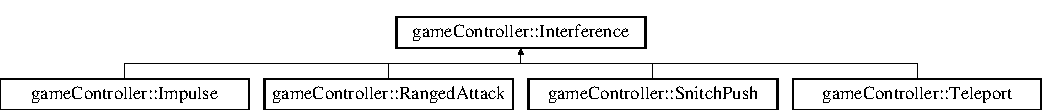
\includegraphics[height=1.473684cm]{classgame_controller_1_1_interference}
\end{center}
\end{figure}
\subsection*{Public Member Functions}
\begin{DoxyCompactItemize}
\item 
\hypertarget{classgame_controller_1_1_interference_a1e664266c768fafd6fc4339e08741d5a}{{\bfseries Interference} (std\-::shared\-\_\-ptr$<$ \hyperlink{classgame_model_1_1_environment}{game\-Model\-::\-Environment} $>$ env, std\-::shared\-\_\-ptr$<$ \hyperlink{classgame_model_1_1_team}{game\-Model\-::\-Team} $>$ team, game\-Model\-::\-Interference\-Type type)}\label{classgame_controller_1_1_interference_a1e664266c768fafd6fc4339e08741d5a}

\item 
virtual void \hyperlink{classgame_controller_1_1_interference_aa5ced37bf22486e1cc290bc6679c2db2}{execute} () const =0
\item 
virtual bool \hyperlink{classgame_controller_1_1_interference_a06b9adc5df035e184e7ed0cf5d4a8814}{is\-Possible} () const 
\item 
auto \hyperlink{classgame_controller_1_1_interference_a694aa2cd65bbb35c02f1ca4ed7701ebe}{get\-Type} () const -\/$>$ game\-Model\-::\-Interference\-Type
\end{DoxyCompactItemize}
\subsection*{Protected Attributes}
\begin{DoxyCompactItemize}
\item 
\hypertarget{classgame_controller_1_1_interference_a599512f23ad5bca74521b15309ea4b88}{std\-::shared\-\_\-ptr\\*
$<$ \hyperlink{classgame_model_1_1_environment}{game\-Model\-::\-Environment} $>$ {\bfseries env}}\label{classgame_controller_1_1_interference_a599512f23ad5bca74521b15309ea4b88}

\item 
\hypertarget{classgame_controller_1_1_interference_aed7a76226c2b0b99e896bcd45d9adc74}{std\-::shared\-\_\-ptr$<$ \hyperlink{classgame_model_1_1_team}{game\-Model\-::\-Team} $>$ {\bfseries team}}\label{classgame_controller_1_1_interference_aed7a76226c2b0b99e896bcd45d9adc74}

\item 
\hypertarget{classgame_controller_1_1_interference_af7bd9e6bb2f92cb4f547ca4f52e5f16c}{game\-Model\-::\-Interference\-Type {\bfseries type}}\label{classgame_controller_1_1_interference_af7bd9e6bb2f92cb4f547ca4f52e5f16c}

\end{DoxyCompactItemize}


\subsection{Member Function Documentation}
\hypertarget{classgame_controller_1_1_interference_aa5ced37bf22486e1cc290bc6679c2db2}{\index{game\-Controller\-::\-Interference@{game\-Controller\-::\-Interference}!execute@{execute}}
\index{execute@{execute}!gameController::Interference@{game\-Controller\-::\-Interference}}
\subsubsection[{execute}]{\setlength{\rightskip}{0pt plus 5cm}virtual void game\-Controller\-::\-Interference\-::execute (
\begin{DoxyParamCaption}
{}
\end{DoxyParamCaption}
) const\hspace{0.3cm}{\ttfamily [pure virtual]}}}\label{classgame_controller_1_1_interference_aa5ced37bf22486e1cc290bc6679c2db2}
Executes the interference 

Implemented in \hyperlink{classgame_controller_1_1_snitch_push_a3abfb90f1d21c8b51971d75012485af4}{game\-Controller\-::\-Snitch\-Push}, \hyperlink{classgame_controller_1_1_impulse_aec92c13c5a3a55da3f8d948354a9b4f4}{game\-Controller\-::\-Impulse}, \hyperlink{classgame_controller_1_1_ranged_attack_a581a62b0f86ef2d510c17cd896382b46}{game\-Controller\-::\-Ranged\-Attack}, and \hyperlink{classgame_controller_1_1_teleport_a9e10c37934bf7447f1cee64545fbf138}{game\-Controller\-::\-Teleport}.

\hypertarget{classgame_controller_1_1_interference_a694aa2cd65bbb35c02f1ca4ed7701ebe}{\index{game\-Controller\-::\-Interference@{game\-Controller\-::\-Interference}!get\-Type@{get\-Type}}
\index{get\-Type@{get\-Type}!gameController::Interference@{game\-Controller\-::\-Interference}}
\subsubsection[{get\-Type}]{\setlength{\rightskip}{0pt plus 5cm}auto game\-Controller\-::\-Interference\-::get\-Type (
\begin{DoxyParamCaption}
{}
\end{DoxyParamCaption}
) const -\/$>$ game\-Model\-::\-Interference\-Type}}\label{classgame_controller_1_1_interference_a694aa2cd65bbb35c02f1ca4ed7701ebe}
Gets the type of interference \begin{DoxyReturn}{Returns}

\end{DoxyReturn}
\hypertarget{classgame_controller_1_1_interference_a06b9adc5df035e184e7ed0cf5d4a8814}{\index{game\-Controller\-::\-Interference@{game\-Controller\-::\-Interference}!is\-Possible@{is\-Possible}}
\index{is\-Possible@{is\-Possible}!gameController::Interference@{game\-Controller\-::\-Interference}}
\subsubsection[{is\-Possible}]{\setlength{\rightskip}{0pt plus 5cm}bool game\-Controller\-::\-Interference\-::is\-Possible (
\begin{DoxyParamCaption}
{}
\end{DoxyParamCaption}
) const\hspace{0.3cm}{\ttfamily [virtual]}}}\label{classgame_controller_1_1_interference_a06b9adc5df035e184e7ed0cf5d4a8814}
Checks if the interference is possible \begin{DoxyReturn}{Returns}

\end{DoxyReturn}


Reimplemented in \hyperlink{classgame_controller_1_1_ranged_attack_a95776ac1efedefee37dd42acd5308e6b}{game\-Controller\-::\-Ranged\-Attack}.



The documentation for this class was generated from the following files\-:\begin{DoxyCompactItemize}
\item 
/home/travis/build/\-So\-Pra-\/\-Team-\/10/\-Game\-Logic/Interference.\-h\item 
/home/travis/build/\-So\-Pra-\/\-Team-\/10/\-Game\-Logic/Interference.\-cpp\end{DoxyCompactItemize}

\hypertarget{classgame_model_1_1_keeper}{\section{game\-Model\-:\-:Keeper Class Reference}
\label{classgame_model_1_1_keeper}\index{game\-Model\-::\-Keeper@{game\-Model\-::\-Keeper}}
}
Inheritance diagram for game\-Model\-:\-:Keeper\-:\begin{figure}[H]
\begin{center}
\leavevmode
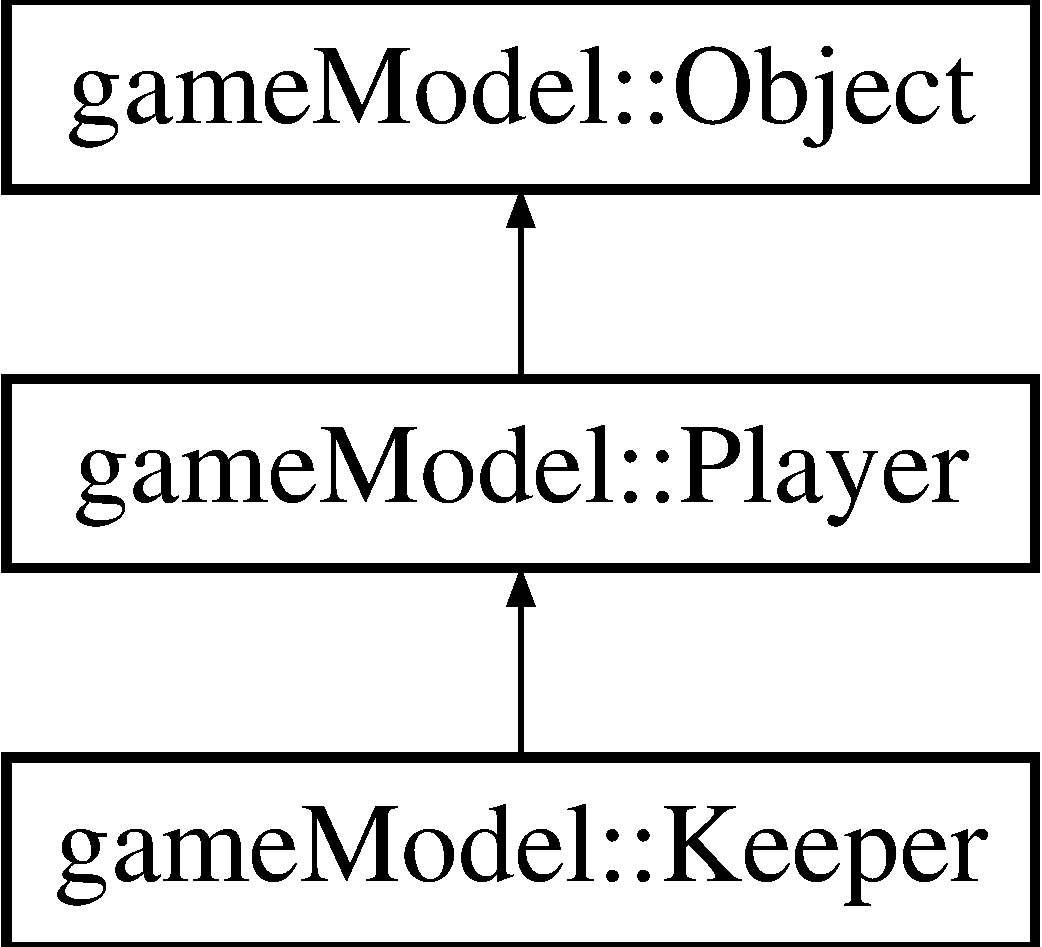
\includegraphics[height=3.000000cm]{classgame_model_1_1_keeper}
\end{center}
\end{figure}
\subsection*{Public Member Functions}
\begin{DoxyCompactItemize}
\item 
\hypertarget{classgame_model_1_1_keeper_ad35a2ca0aee3f986e6287973b7786a88}{{\bfseries Keeper} (\hyperlink{structgame_model_1_1_position}{Position} position, std\-::string name, communication\-::messages\-::types\-::\-Sex gender, communication\-::messages\-::types\-::\-Broom broom, communication\-::messages\-::types\-::\-Entity\-Id id)}\label{classgame_model_1_1_keeper_ad35a2ca0aee3f986e6287973b7786a88}

\end{DoxyCompactItemize}
\subsection*{Additional Inherited Members}


The documentation for this class was generated from the following file\-:\begin{DoxyCompactItemize}
\item 
/home/travis/build/\-So\-Pra-\/\-Team-\/10/\-Game\-Logic/Game\-Model.\-h\end{DoxyCompactItemize}

\hypertarget{classgame_controller_1_1_move}{\section{game\-Controller\-:\-:Move Class Reference}
\label{classgame_controller_1_1_move}\index{game\-Controller\-::\-Move@{game\-Controller\-::\-Move}}
}


{\ttfamily \#include $<$Action.\-h$>$}

Inheritance diagram for game\-Controller\-:\-:Move\-:\begin{figure}[H]
\begin{center}
\leavevmode
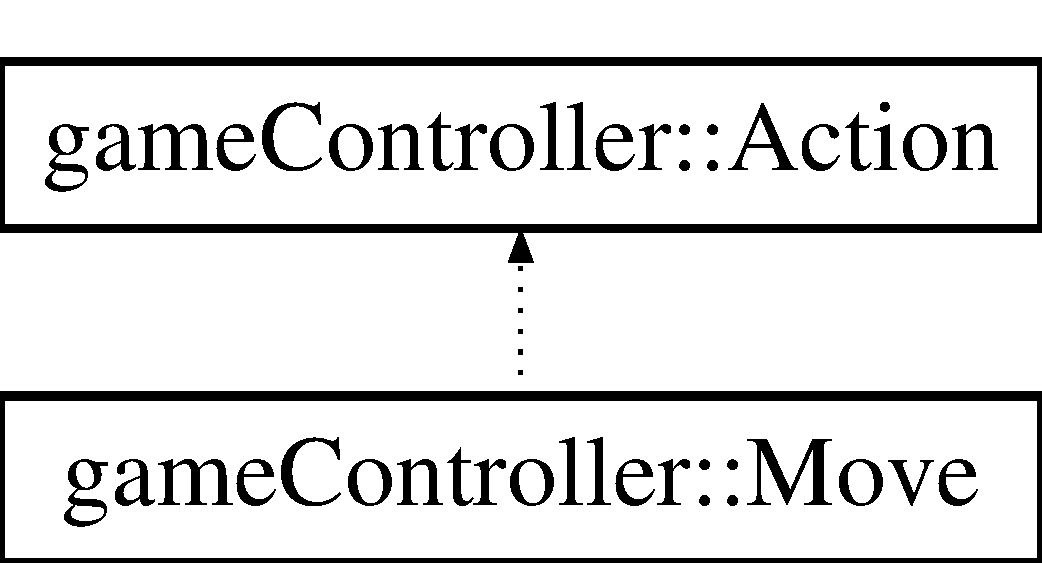
\includegraphics[height=2.000000cm]{classgame_controller_1_1_move}
\end{center}
\end{figure}
\subsection*{Public Member Functions}
\begin{DoxyCompactItemize}
\item 
\hyperlink{classgame_controller_1_1_move_a7336aaeac611eaa78bfeb93d978f9e7c}{Move} ()=default
\item 
\hyperlink{classgame_controller_1_1_move_a6b27870ecb6182853feb7607c78bd5bb}{Move} (std\-::shared\-\_\-ptr$<$ \hyperlink{classgame_model_1_1_environment}{game\-Model\-::\-Environment} $>$ env, std\-::shared\-\_\-ptr$<$ \hyperlink{classgame_model_1_1_player}{game\-Model\-::\-Player} $>$ actor, \hyperlink{structgame_model_1_1_position}{game\-Model\-::\-Position} target)
\item 
auto \hyperlink{classgame_controller_1_1_move_a57822a002472b25276be2a6678569f72}{execute} () const -\/$>$ std\-::pair$<$ std\-::vector$<$ Shot\-Result $>$, std\-::vector$<$ game\-Model\-::\-Foul $>$$>$
\item 
auto \hyperlink{classgame_controller_1_1_move_ae36dc4d09881c114cc8c9192e6f85988}{success\-Prob} () const -\/$>$ double override
\item 
auto \hyperlink{classgame_controller_1_1_move_a5ff9c2a76dbfdc59a0dd206b74279be0}{check} () const -\/$>$ Action\-Check\-Result override
\item 
auto \hyperlink{classgame_controller_1_1_move_a3b9266d42dfc66fe16c228a08927cb8a}{execute\-All} () const -\/$>$ std\-::vector$<$ std\-::pair$<$ \hyperlink{classgame_model_1_1_environment}{game\-Model\-::\-Environment}, double $>$$>$ override
\item 
auto \hyperlink{classgame_controller_1_1_move_acf276f2198a6229660727956a5f156ad}{check\-For\-Foul} () const -\/$>$ std\-::vector$<$ game\-Model\-::\-Foul $>$
\end{DoxyCompactItemize}


\subsection{Detailed Description}
class for a move in the game which can be executed by a player or a ball 

\subsection{Constructor \& Destructor Documentation}
\hypertarget{classgame_controller_1_1_move_a7336aaeac611eaa78bfeb93d978f9e7c}{\index{game\-Controller\-::\-Move@{game\-Controller\-::\-Move}!Move@{Move}}
\index{Move@{Move}!gameController::Move@{game\-Controller\-::\-Move}}
\subsubsection[{Move}]{\setlength{\rightskip}{0pt plus 5cm}game\-Controller\-::\-Move\-::\-Move (
\begin{DoxyParamCaption}
{}
\end{DoxyParamCaption}
)\hspace{0.3cm}{\ttfamily [default]}}}\label{classgame_controller_1_1_move_a7336aaeac611eaa78bfeb93d978f9e7c}
default constructor for the \hyperlink{classgame_controller_1_1_move}{Move} Class. \hypertarget{classgame_controller_1_1_move_a6b27870ecb6182853feb7607c78bd5bb}{\index{game\-Controller\-::\-Move@{game\-Controller\-::\-Move}!Move@{Move}}
\index{Move@{Move}!gameController::Move@{game\-Controller\-::\-Move}}
\subsubsection[{Move}]{\setlength{\rightskip}{0pt plus 5cm}game\-Controller\-::\-Move\-::\-Move (
\begin{DoxyParamCaption}
\item[{std\-::shared\-\_\-ptr$<$ {\bf game\-Model\-::\-Environment} $>$}]{env, }
\item[{std\-::shared\-\_\-ptr$<$ {\bf game\-Model\-::\-Player} $>$}]{actor, }
\item[{{\bf game\-Model\-::\-Position}}]{target}
\end{DoxyParamCaption}
)}}\label{classgame_controller_1_1_move_a6b27870ecb6182853feb7607c78bd5bb}
main constructor for the \hyperlink{classgame_controller_1_1_move}{Move} class. 
\begin{DoxyParams}{Parameters}
{\em env} & the environment to operate on \\
\hline
{\em actor} & the acting player or ball as shared pointer. \\
\hline
{\em target} & the target position of the move. \\
\hline
\end{DoxyParams}


\subsection{Member Function Documentation}
\hypertarget{classgame_controller_1_1_move_a5ff9c2a76dbfdc59a0dd206b74279be0}{\index{game\-Controller\-::\-Move@{game\-Controller\-::\-Move}!check@{check}}
\index{check@{check}!gameController::Move@{game\-Controller\-::\-Move}}
\subsubsection[{check}]{\setlength{\rightskip}{0pt plus 5cm}auto game\-Controller\-::\-Move\-::check (
\begin{DoxyParamCaption}
{}
\end{DoxyParamCaption}
) const -\/$>$ Action\-Check\-Result\hspace{0.3cm}{\ttfamily [override]}, {\ttfamily [virtual]}}}\label{classgame_controller_1_1_move_a5ff9c2a76dbfdc59a0dd206b74279be0}
check if the selected move is possible (implementation of virtual function) 
\begin{DoxyParams}{Parameters}
{\em envi} & the selected environment. \\
\hline
\end{DoxyParams}
\begin{DoxyReturn}{Returns}
the result of the check as Action\-Result. 
\end{DoxyReturn}


Implements \hyperlink{classgame_controller_1_1_action}{game\-Controller\-::\-Action}.

\hypertarget{classgame_controller_1_1_move_acf276f2198a6229660727956a5f156ad}{\index{game\-Controller\-::\-Move@{game\-Controller\-::\-Move}!check\-For\-Foul@{check\-For\-Foul}}
\index{check\-For\-Foul@{check\-For\-Foul}!gameController::Move@{game\-Controller\-::\-Move}}
\subsubsection[{check\-For\-Foul}]{\setlength{\rightskip}{0pt plus 5cm}auto game\-Controller\-::\-Move\-::check\-For\-Foul (
\begin{DoxyParamCaption}
{}
\end{DoxyParamCaption}
) const -\/$>$ std\-::vector$<$game\-Model\-::\-Foul$>$}}\label{classgame_controller_1_1_move_acf276f2198a6229660727956a5f156ad}
checks if the move is a foul. 
\begin{DoxyParams}{Parameters}
{\em envi} & the selected environment. \\
\hline
\end{DoxyParams}
\begin{DoxyReturn}{Returns}
the type of foul. 
\end{DoxyReturn}
\hypertarget{classgame_controller_1_1_move_a57822a002472b25276be2a6678569f72}{\index{game\-Controller\-::\-Move@{game\-Controller\-::\-Move}!execute@{execute}}
\index{execute@{execute}!gameController::Move@{game\-Controller\-::\-Move}}
\subsubsection[{execute}]{\setlength{\rightskip}{0pt plus 5cm}auto game\-Controller\-::\-Move\-::execute (
\begin{DoxyParamCaption}
{}
\end{DoxyParamCaption}
) const -\/$>$ std\-::pair$<$std\-::vector$<$Shot\-Result$>$, std\-::vector$<$game\-Model\-::\-Foul$>$$>$\hspace{0.3cm}{\ttfamily [virtual]}}}\label{classgame_controller_1_1_move_a57822a002472b25276be2a6678569f72}
execute the move in a given environment (implementation of virtual function). 
\begin{DoxyParams}{Parameters}
{\em envi} & the environment in which the shot should be performed. \\
\hline
\end{DoxyParams}


Implements \hyperlink{classgame_controller_1_1_action}{game\-Controller\-::\-Action}.

\hypertarget{classgame_controller_1_1_move_a3b9266d42dfc66fe16c228a08927cb8a}{\index{game\-Controller\-::\-Move@{game\-Controller\-::\-Move}!execute\-All@{execute\-All}}
\index{execute\-All@{execute\-All}!gameController::Move@{game\-Controller\-::\-Move}}
\subsubsection[{execute\-All}]{\setlength{\rightskip}{0pt plus 5cm}auto game\-Controller\-::\-Move\-::execute\-All (
\begin{DoxyParamCaption}
{}
\end{DoxyParamCaption}
) const -\/$>$ std\-::vector$<$std\-::pair$<${\bf game\-Model\-::\-Environment}, double$>$$>$\hspace{0.3cm}{\ttfamily [override]}, {\ttfamily [virtual]}}}\label{classgame_controller_1_1_move_a3b9266d42dfc66fe16c228a08927cb8a}
execute all given move in a given environment (implementation of virtual function). 
\begin{DoxyParams}{Parameters}
{\em envi} & the selected environment. \\
\hline
\end{DoxyParams}
\begin{DoxyReturn}{Returns}
the resulting environments an there probabilities as a pair. 
\end{DoxyReturn}


Implements \hyperlink{classgame_controller_1_1_action}{game\-Controller\-::\-Action}.

\hypertarget{classgame_controller_1_1_move_ae36dc4d09881c114cc8c9192e6f85988}{\index{game\-Controller\-::\-Move@{game\-Controller\-::\-Move}!success\-Prob@{success\-Prob}}
\index{success\-Prob@{success\-Prob}!gameController::Move@{game\-Controller\-::\-Move}}
\subsubsection[{success\-Prob}]{\setlength{\rightskip}{0pt plus 5cm}auto game\-Controller\-::\-Move\-::success\-Prob (
\begin{DoxyParamCaption}
{}
\end{DoxyParamCaption}
) const -\/$>$ double\hspace{0.3cm}{\ttfamily [override]}, {\ttfamily [virtual]}}}\label{classgame_controller_1_1_move_ae36dc4d09881c114cc8c9192e6f85988}
get the success probability of the move (implementation of virtual function). (implementation of virtual function). \begin{DoxyReturn}{Returns}
the success probability of the move as double. 
\end{DoxyReturn}


Implements \hyperlink{classgame_controller_1_1_action}{game\-Controller\-::\-Action}.



The documentation for this class was generated from the following files\-:\begin{DoxyCompactItemize}
\item 
/home/travis/build/\-So\-Pra-\/\-Team-\/10/\-Game\-Logic/Action.\-h\item 
/home/travis/build/\-So\-Pra-\/\-Team-\/10/\-Game\-Logic/Action.\-cpp\end{DoxyCompactItemize}

\hypertarget{classgame_model_1_1_object}{\section{game\-Model\-:\-:Object Class Reference}
\label{classgame_model_1_1_object}\index{game\-Model\-::\-Object@{game\-Model\-::\-Object}}
}
Inheritance diagram for game\-Model\-:\-:Object\-:\begin{figure}[H]
\begin{center}
\leavevmode
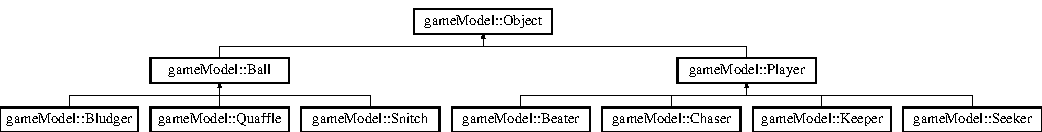
\includegraphics[height=1.777778cm]{classgame_model_1_1_object}
\end{center}
\end{figure}
\subsection*{Public Member Functions}
\begin{DoxyCompactItemize}
\item 
\hypertarget{classgame_model_1_1_object_a22ec074a1b4f4c3b90e0827b07939f10}{{\bfseries Object} (const \hyperlink{structgame_model_1_1_position}{Position} \&position, communication\-::messages\-::types\-::\-Entity\-Id id)}\label{classgame_model_1_1_object_a22ec074a1b4f4c3b90e0827b07939f10}

\end{DoxyCompactItemize}
\subsection*{Data Fields}
\begin{DoxyCompactItemize}
\item 
\hypertarget{classgame_model_1_1_object_a852c8ff1e230a07349aa8dc60b8cbd71}{\hyperlink{structgame_model_1_1_position}{Position} {\bfseries position} = \{\}}\label{classgame_model_1_1_object_a852c8ff1e230a07349aa8dc60b8cbd71}

\item 
\hypertarget{classgame_model_1_1_object_ada26da82f66b6139d4a430962ebbef22}{const \\*
communication\-::messages\-::types\-::\-Entity\-Id {\bfseries id} \{\}}\label{classgame_model_1_1_object_ada26da82f66b6139d4a430962ebbef22}

\end{DoxyCompactItemize}


The documentation for this class was generated from the following files\-:\begin{DoxyCompactItemize}
\item 
/home/travis/build/\-So\-Pra-\/\-Team-\/10/\-Game\-Logic/Game\-Model.\-h\item 
/home/travis/build/\-So\-Pra-\/\-Team-\/10/\-Game\-Logic/Game\-Model.\-cpp\end{DoxyCompactItemize}

\hypertarget{classgame_model_1_1_player}{\section{game\-Model\-:\-:Player Class Reference}
\label{classgame_model_1_1_player}\index{game\-Model\-::\-Player@{game\-Model\-::\-Player}}
}


{\ttfamily \#include $<$Game\-Model.\-h$>$}

Inheritance diagram for game\-Model\-:\-:Player\-:\begin{figure}[H]
\begin{center}
\leavevmode
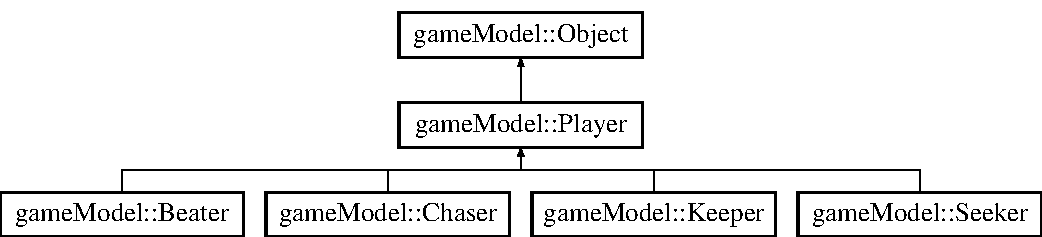
\includegraphics[height=3.000000cm]{classgame_model_1_1_player}
\end{center}
\end{figure}
\subsection*{Public Member Functions}
\begin{DoxyCompactItemize}
\item 
\hypertarget{classgame_model_1_1_player_a2c01b78c33c808ff91919f8af0ee7023}{{\bfseries Player} (\hyperlink{structgame_model_1_1_position}{Position} position, std\-::string name, communication\-::messages\-::types\-::\-Sex gender, communication\-::messages\-::types\-::\-Broom broom, communication\-::messages\-::types\-::\-Entity\-Id id)}\label{classgame_model_1_1_player_a2c01b78c33c808ff91919f8af0ee7023}

\item 
\hypertarget{classgame_model_1_1_player_a834398ab0d22ebed1c174cf68b8ed115}{bool {\bfseries operator==} (const \hyperlink{classgame_model_1_1_player}{Player} \&other) const }\label{classgame_model_1_1_player_a834398ab0d22ebed1c174cf68b8ed115}

\item 
\hypertarget{classgame_model_1_1_player_ae7e2df45f035fa1ea2971b21bb15b001}{bool {\bfseries operator!=} (const \hyperlink{classgame_model_1_1_player}{Player} \&other) const }\label{classgame_model_1_1_player_ae7e2df45f035fa1ea2971b21bb15b001}

\end{DoxyCompactItemize}
\subsection*{Data Fields}
\begin{DoxyCompactItemize}
\item 
\hypertarget{classgame_model_1_1_player_a2ec251df1a0164889083c2c4efee89f5}{std\-::string {\bfseries name}}\label{classgame_model_1_1_player_a2ec251df1a0164889083c2c4efee89f5}

\item 
\hypertarget{classgame_model_1_1_player_a6b07ad3fedeec2dfc4854d97118dafa8}{communication\-::messages\-::types\-::\-Sex {\bfseries gender} = \{\}}\label{classgame_model_1_1_player_a6b07ad3fedeec2dfc4854d97118dafa8}

\item 
\hypertarget{classgame_model_1_1_player_ae9ce9fdb6971621553a501c99d12ed6f}{communication\-::messages\-::types\-::\-Broom {\bfseries broom} = \{\}}\label{classgame_model_1_1_player_ae9ce9fdb6971621553a501c99d12ed6f}

\item 
\hypertarget{classgame_model_1_1_player_ad0cbf1657de62c39c4101a9d7f2398c6}{bool {\bfseries is\-Fined} = false}\label{classgame_model_1_1_player_ad0cbf1657de62c39c4101a9d7f2398c6}

\item 
\hypertarget{classgame_model_1_1_player_aa638922565fbdc4044b65467cc8e1d11}{bool {\bfseries knocked\-Out} = false}\label{classgame_model_1_1_player_aa638922565fbdc4044b65467cc8e1d11}

\end{DoxyCompactItemize}


\subsection{Detailed Description}
Represents the playable characters 

The documentation for this class was generated from the following files\-:\begin{DoxyCompactItemize}
\item 
/home/travis/build/\-So\-Pra-\/\-Team-\/10/\-Game\-Logic/Game\-Model.\-h\item 
/home/travis/build/\-So\-Pra-\/\-Team-\/10/\-Game\-Logic/Game\-Model.\-cpp\end{DoxyCompactItemize}

\hypertarget{structgame_model_1_1_position}{\section{game\-Model\-:\-:Position Struct Reference}
\label{structgame_model_1_1_position}\index{game\-Model\-::\-Position@{game\-Model\-::\-Position}}
}


{\ttfamily \#include $<$Game\-Model.\-h$>$}

\subsection*{Public Member Functions}
\begin{DoxyCompactItemize}
\item 
\hypertarget{structgame_model_1_1_position_adb34a80ed89108f40a0d642fdbdd4e44}{{\bfseries Position} (int x, int y)}\label{structgame_model_1_1_position_adb34a80ed89108f40a0d642fdbdd4e44}

\item 
\hypertarget{structgame_model_1_1_position_aa2d124ca5ef188d18a71dac9620c8113}{bool {\bfseries operator==} (const \hyperlink{structgame_model_1_1_position}{Position} \&other) const }\label{structgame_model_1_1_position_aa2d124ca5ef188d18a71dac9620c8113}

\item 
\hypertarget{structgame_model_1_1_position_a8517d6cf475cc8110f81036caf60dde9}{bool {\bfseries operator!=} (const \hyperlink{structgame_model_1_1_position}{Position} \&other) const }\label{structgame_model_1_1_position_a8517d6cf475cc8110f81036caf60dde9}

\end{DoxyCompactItemize}
\subsection*{Data Fields}
\begin{DoxyCompactItemize}
\item 
\hypertarget{structgame_model_1_1_position_a8b8c016c29a18d0c6a8668498f063845}{int {\bfseries x}}\label{structgame_model_1_1_position_a8b8c016c29a18d0c6a8668498f063845}

\item 
\hypertarget{structgame_model_1_1_position_ac17e5a319be555282b38655ee00a6e07}{int {\bfseries y}}\label{structgame_model_1_1_position_ac17e5a319be555282b38655ee00a6e07}

\end{DoxyCompactItemize}


\subsection{Detailed Description}
This struct represents a 2\-D-\/\-Position on the Gamefield 

The documentation for this struct was generated from the following files\-:\begin{DoxyCompactItemize}
\item 
/home/travis/build/\-So\-Pra-\/\-Team-\/10/\-Game\-Logic/Game\-Model.\-h\item 
/home/travis/build/\-So\-Pra-\/\-Team-\/10/\-Game\-Logic/Game\-Model.\-cpp\end{DoxyCompactItemize}

\hypertarget{classgame_model_1_1_quaffle}{\section{game\-Model\-:\-:Quaffle Class Reference}
\label{classgame_model_1_1_quaffle}\index{game\-Model\-::\-Quaffle@{game\-Model\-::\-Quaffle}}
}
Inheritance diagram for game\-Model\-:\-:Quaffle\-:\begin{figure}[H]
\begin{center}
\leavevmode
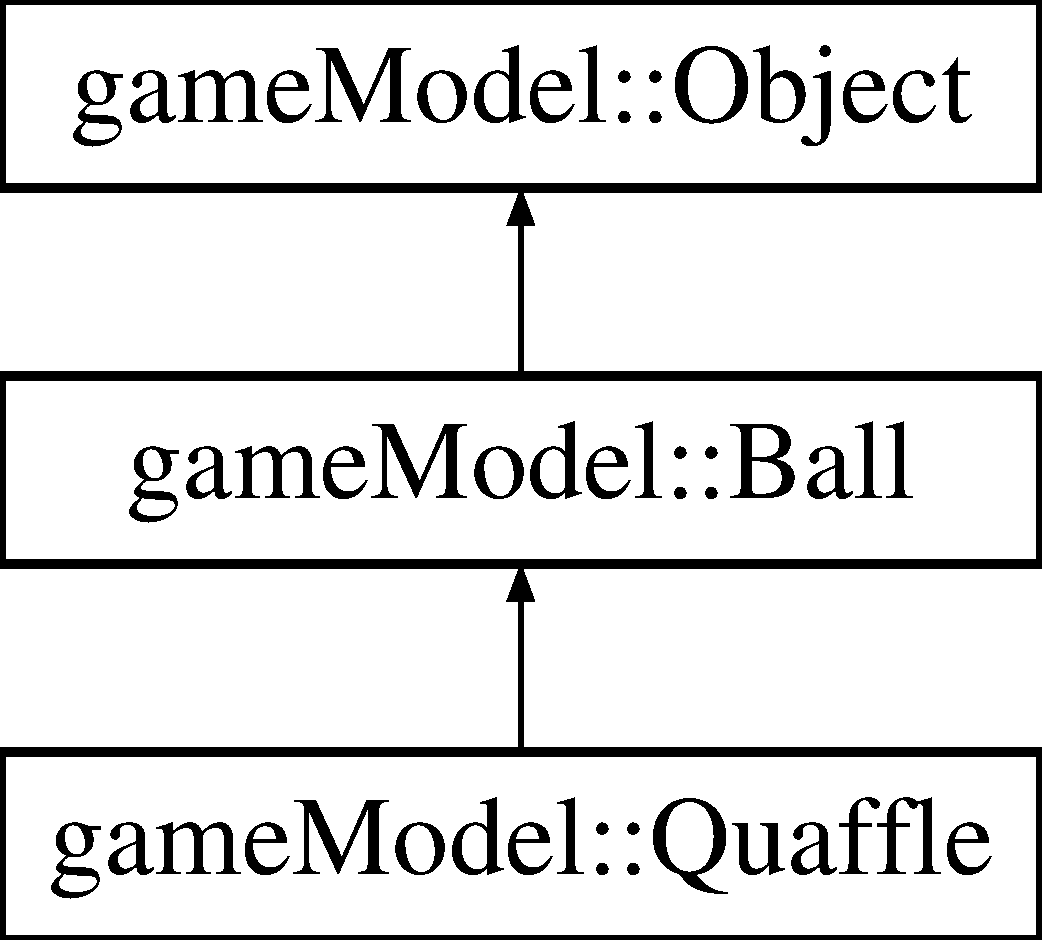
\includegraphics[height=3.000000cm]{classgame_model_1_1_quaffle}
\end{center}
\end{figure}
\subsection*{Public Member Functions}
\begin{DoxyCompactItemize}
\item 
\hyperlink{classgame_model_1_1_quaffle_af7edb1afbd12237b3c86ab21d0f830f1}{Quaffle} ()
\item 
\hypertarget{classgame_model_1_1_quaffle_a3f20c2b1efd5874b6cee2563a0f73f1f}{{\bfseries Quaffle} (\hyperlink{structgame_model_1_1_position}{Position} position)}\label{classgame_model_1_1_quaffle_a3f20c2b1efd5874b6cee2563a0f73f1f}

\end{DoxyCompactItemize}
\subsection*{Additional Inherited Members}


\subsection{Constructor \& Destructor Documentation}
\hypertarget{classgame_model_1_1_quaffle_af7edb1afbd12237b3c86ab21d0f830f1}{\index{game\-Model\-::\-Quaffle@{game\-Model\-::\-Quaffle}!Quaffle@{Quaffle}}
\index{Quaffle@{Quaffle}!gameModel::Quaffle@{game\-Model\-::\-Quaffle}}
\subsubsection[{Quaffle}]{\setlength{\rightskip}{0pt plus 5cm}game\-Model\-::\-Quaffle\-::\-Quaffle (
\begin{DoxyParamCaption}
{}
\end{DoxyParamCaption}
)}}\label{classgame_model_1_1_quaffle_af7edb1afbd12237b3c86ab21d0f830f1}
Places \hyperlink{classgame_model_1_1_quaffle}{Quaffle} in the centre of the field 

The documentation for this class was generated from the following file\-:\begin{DoxyCompactItemize}
\item 
/home/travis/build/\-So\-Pra-\/\-Team-\/10/\-Game\-Logic/Game\-Model.\-h\end{DoxyCompactItemize}

\hypertarget{classgame_controller_1_1_ranged_attack}{\section{game\-Controller\-:\-:Ranged\-Attack Class Reference}
\label{classgame_controller_1_1_ranged_attack}\index{game\-Controller\-::\-Ranged\-Attack@{game\-Controller\-::\-Ranged\-Attack}}
}
Inheritance diagram for game\-Controller\-:\-:Ranged\-Attack\-:\begin{figure}[H]
\begin{center}
\leavevmode
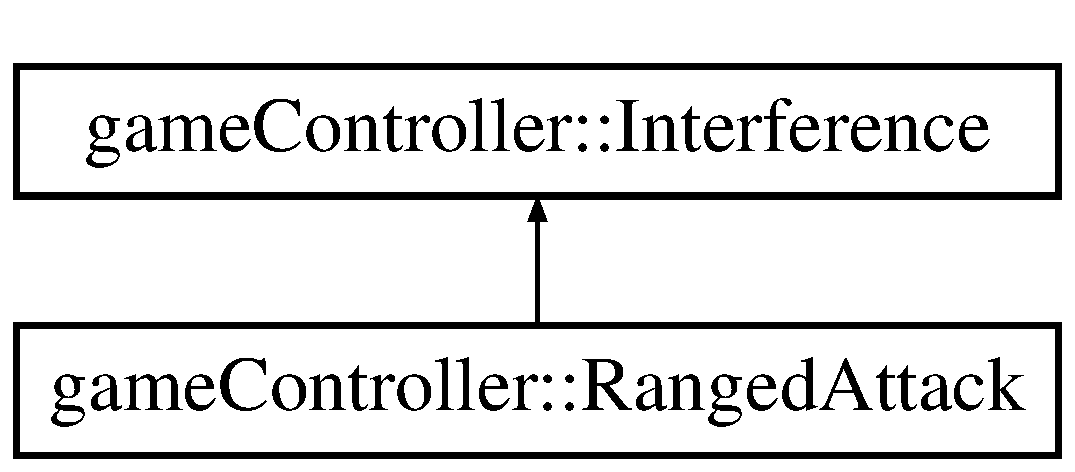
\includegraphics[height=2.000000cm]{classgame_controller_1_1_ranged_attack}
\end{center}
\end{figure}
\subsection*{Public Member Functions}
\begin{DoxyCompactItemize}
\item 
\hypertarget{classgame_controller_1_1_ranged_attack_a467d9e5a0c8e6c19b3f3214bc3781c19}{{\bfseries Ranged\-Attack} (std\-::shared\-\_\-ptr$<$ \hyperlink{classgame_model_1_1_environment}{game\-Model\-::\-Environment} $>$ env, std\-::shared\-\_\-ptr$<$ \hyperlink{classgame_model_1_1_team}{game\-Model\-::\-Team} $>$ team, std\-::shared\-\_\-ptr$<$ \hyperlink{classgame_model_1_1_player}{game\-Model\-::\-Player} $>$ target)}\label{classgame_controller_1_1_ranged_attack_a467d9e5a0c8e6c19b3f3214bc3781c19}

\item 
auto \hyperlink{classgame_controller_1_1_ranged_attack_a7c5cb7567f7f6bc8fb844837240d7c09}{execute} () const -\/$>$ game\-Controller\-::\-Action\-Check\-Result override
\item 
bool \hyperlink{classgame_controller_1_1_ranged_attack_a95776ac1efedefee37dd42acd5308e6b}{is\-Possible} () const override
\end{DoxyCompactItemize}
\subsection*{Additional Inherited Members}


\subsection{Member Function Documentation}
\hypertarget{classgame_controller_1_1_ranged_attack_a7c5cb7567f7f6bc8fb844837240d7c09}{\index{game\-Controller\-::\-Ranged\-Attack@{game\-Controller\-::\-Ranged\-Attack}!execute@{execute}}
\index{execute@{execute}!gameController::RangedAttack@{game\-Controller\-::\-Ranged\-Attack}}
\subsubsection[{execute}]{\setlength{\rightskip}{0pt plus 5cm}auto game\-Controller\-::\-Ranged\-Attack\-::execute (
\begin{DoxyParamCaption}
{}
\end{DoxyParamCaption}
) const -\/$>$ game\-Controller\-::\-Action\-Check\-Result\hspace{0.3cm}{\ttfamily [override]}, {\ttfamily [virtual]}}}\label{classgame_controller_1_1_ranged_attack_a7c5cb7567f7f6bc8fb844837240d7c09}
Pushes target player to a random free adjacent position if target player previously held quaffle, quaffle will be moved to random free adjacent position 

Implements \hyperlink{classgame_controller_1_1_interference_aee66a8480fccc6286b5bef04777a8a6a}{game\-Controller\-::\-Interference}.

\hypertarget{classgame_controller_1_1_ranged_attack_a95776ac1efedefee37dd42acd5308e6b}{\index{game\-Controller\-::\-Ranged\-Attack@{game\-Controller\-::\-Ranged\-Attack}!is\-Possible@{is\-Possible}}
\index{is\-Possible@{is\-Possible}!gameController::RangedAttack@{game\-Controller\-::\-Ranged\-Attack}}
\subsubsection[{is\-Possible}]{\setlength{\rightskip}{0pt plus 5cm}bool game\-Controller\-::\-Ranged\-Attack\-::is\-Possible (
\begin{DoxyParamCaption}
{}
\end{DoxyParamCaption}
) const\hspace{0.3cm}{\ttfamily [override]}, {\ttfamily [virtual]}}}\label{classgame_controller_1_1_ranged_attack_a95776ac1efedefee37dd42acd5308e6b}
\begin{DoxyReturn}{Returns}
true if available and opponent target, false otherwise 
\end{DoxyReturn}


Reimplemented from \hyperlink{classgame_controller_1_1_interference_a06b9adc5df035e184e7ed0cf5d4a8814}{game\-Controller\-::\-Interference}.



The documentation for this class was generated from the following files\-:\begin{DoxyCompactItemize}
\item 
/home/travis/build/\-So\-Pra-\/\-Team-\/10/\-Game\-Logic/Interference.\-h\item 
/home/travis/build/\-So\-Pra-\/\-Team-\/10/\-Game\-Logic/Interference.\-cpp\end{DoxyCompactItemize}

\hypertarget{classgame_model_1_1_seeker}{\section{game\-Model\-:\-:Seeker Class Reference}
\label{classgame_model_1_1_seeker}\index{game\-Model\-::\-Seeker@{game\-Model\-::\-Seeker}}
}
Inheritance diagram for game\-Model\-:\-:Seeker\-:\begin{figure}[H]
\begin{center}
\leavevmode
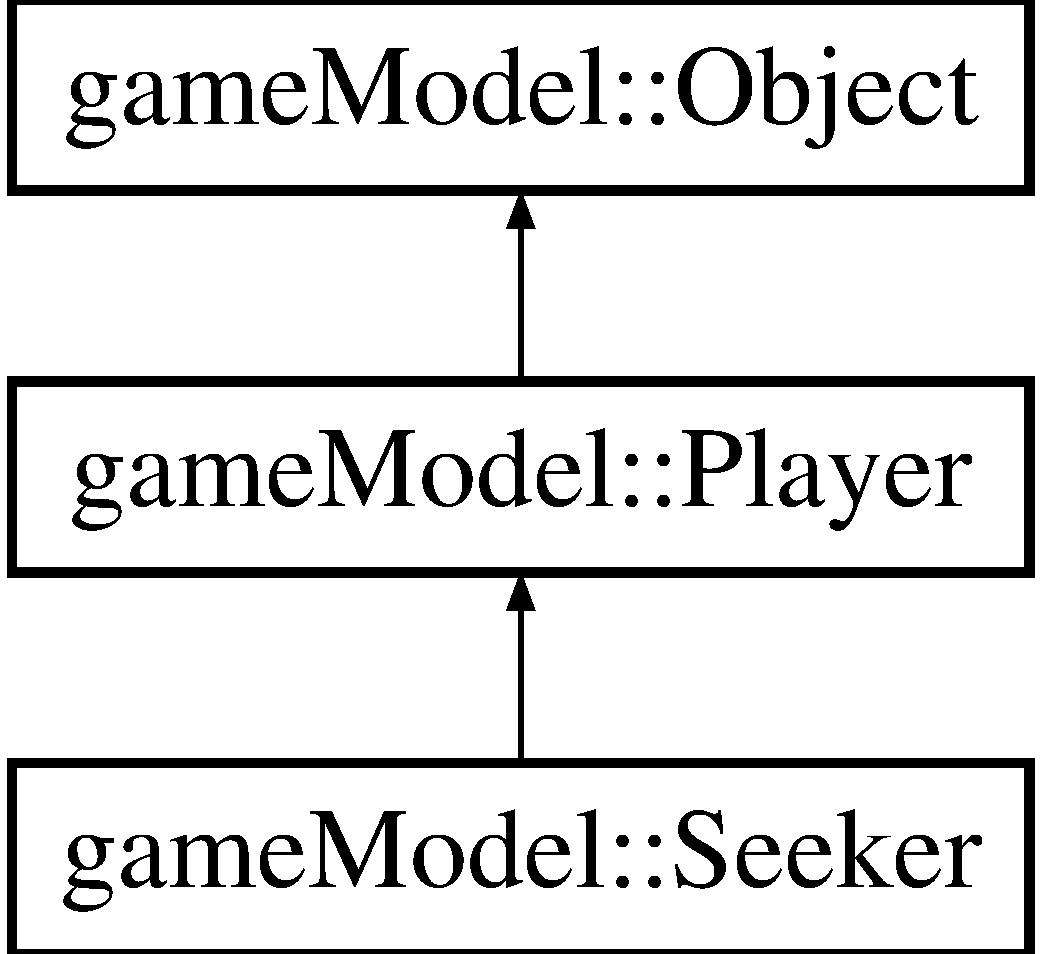
\includegraphics[height=3.000000cm]{classgame_model_1_1_seeker}
\end{center}
\end{figure}
\subsection*{Public Member Functions}
\begin{DoxyCompactItemize}
\item 
\hypertarget{classgame_model_1_1_seeker_aeb98e15de8e8c12a4131d9fb42790d6d}{{\bfseries Seeker} (\hyperlink{structgame_model_1_1_position}{Position} position, std\-::string name, communication\-::messages\-::types\-::\-Sex gender, communication\-::messages\-::types\-::\-Broom broom, communication\-::messages\-::types\-::\-Entity\-Id id)}\label{classgame_model_1_1_seeker_aeb98e15de8e8c12a4131d9fb42790d6d}

\end{DoxyCompactItemize}
\subsection*{Additional Inherited Members}


The documentation for this class was generated from the following file\-:\begin{DoxyCompactItemize}
\item 
/home/travis/build/\-So\-Pra-\/\-Team-\/10/\-Game\-Logic/Game\-Model.\-h\end{DoxyCompactItemize}

\hypertarget{classgame_controller_1_1_shot}{\section{game\-Controller\-:\-:Shot Class Reference}
\label{classgame_controller_1_1_shot}\index{game\-Controller\-::\-Shot@{game\-Controller\-::\-Shot}}
}


{\ttfamily \#include $<$Action.\-h$>$}

Inheritance diagram for game\-Controller\-:\-:Shot\-:\begin{figure}[H]
\begin{center}
\leavevmode
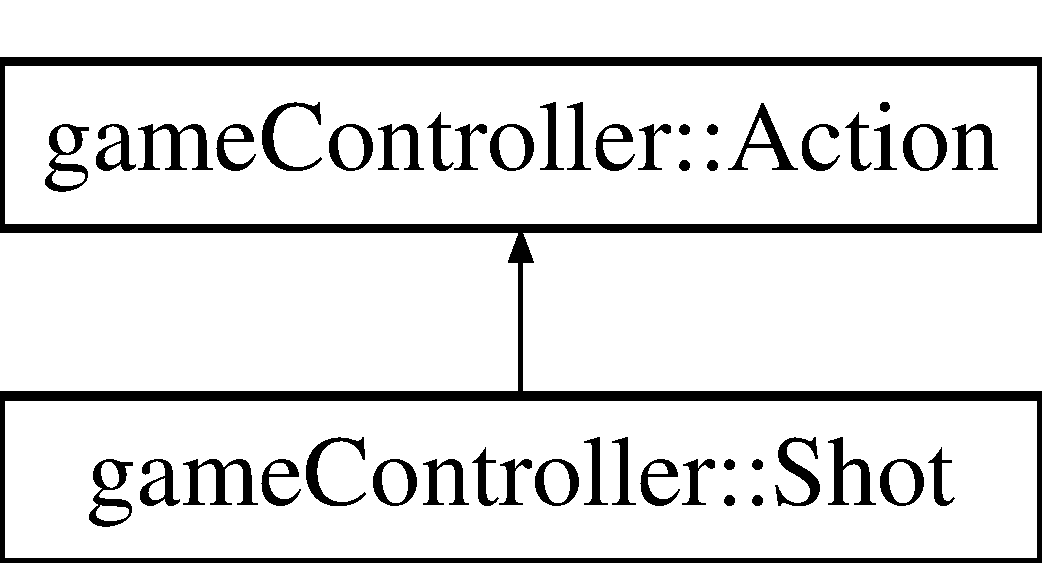
\includegraphics[height=2.000000cm]{classgame_controller_1_1_shot}
\end{center}
\end{figure}
\subsection*{Public Member Functions}
\begin{DoxyCompactItemize}
\item 
\hyperlink{classgame_controller_1_1_shot_a2bb5e375728dc141ef49a0f97dd36def}{Shot} (std\-::shared\-\_\-ptr$<$ \hyperlink{classgame_model_1_1_environment}{game\-Model\-::\-Environment} $>$ env, std\-::shared\-\_\-ptr$<$ \hyperlink{classgame_model_1_1_player}{game\-Model\-::\-Player} $>$ actor, std\-::shared\-\_\-ptr$<$ \hyperlink{classgame_model_1_1_ball}{game\-Model\-::\-Ball} $>$ ball, \hyperlink{structgame_model_1_1_position}{game\-Model\-::\-Position} target)
\item 
auto \hyperlink{classgame_controller_1_1_shot_a88b44fee398655bde62612376e7d2c3d}{execute} () const -\/$>$ std\-::pair$<$ std\-::vector$<$ Shot\-Result $>$, std\-::vector$<$ game\-Model\-::\-Foul $>$$>$
\item 
auto \hyperlink{classgame_controller_1_1_shot_a97b77844c8035c36d6dabfaadcdc0aa7}{success\-Prob} () const -\/$>$ double override
\item 
auto \hyperlink{classgame_controller_1_1_shot_abb3656ea14d64a07d2aef45e6410dfd8}{check} () const -\/$>$ Action\-Check\-Result override
\item 
auto \hyperlink{classgame_controller_1_1_shot_ae595cfcdfc6bb637860e98812df3db67}{execute\-All} () const -\/$>$ std\-::vector$<$ std\-::pair$<$ \hyperlink{classgame_model_1_1_environment}{game\-Model\-::\-Environment}, double $>$$>$ override
\end{DoxyCompactItemize}
\subsection*{Additional Inherited Members}


\subsection{Detailed Description}
class for a shot in the game which can only be executed by a player 

\subsection{Constructor \& Destructor Documentation}
\hypertarget{classgame_controller_1_1_shot_a2bb5e375728dc141ef49a0f97dd36def}{\index{game\-Controller\-::\-Shot@{game\-Controller\-::\-Shot}!Shot@{Shot}}
\index{Shot@{Shot}!gameController::Shot@{game\-Controller\-::\-Shot}}
\subsubsection[{Shot}]{\setlength{\rightskip}{0pt plus 5cm}game\-Controller\-::\-Shot\-::\-Shot (
\begin{DoxyParamCaption}
\item[{std\-::shared\-\_\-ptr$<$ {\bf game\-Model\-::\-Environment} $>$}]{env, }
\item[{std\-::shared\-\_\-ptr$<$ {\bf game\-Model\-::\-Player} $>$}]{actor, }
\item[{std\-::shared\-\_\-ptr$<$ {\bf game\-Model\-::\-Ball} $>$}]{ball, }
\item[{{\bf game\-Model\-::\-Position}}]{target}
\end{DoxyParamCaption}
)}}\label{classgame_controller_1_1_shot_a2bb5e375728dc141ef49a0f97dd36def}
main constructor for the \hyperlink{classgame_controller_1_1_shot}{Shot} class. 
\begin{DoxyParams}{Parameters}
{\em env} & the environment to operate on \\
\hline
{\em actor} & the acting player as shared pointer. \\
\hline
{\em ball} & The ball to be moved \\
\hline
{\em target} & the target position of the shot. \\
\hline
\end{DoxyParams}


\subsection{Member Function Documentation}
\hypertarget{classgame_controller_1_1_shot_abb3656ea14d64a07d2aef45e6410dfd8}{\index{game\-Controller\-::\-Shot@{game\-Controller\-::\-Shot}!check@{check}}
\index{check@{check}!gameController::Shot@{game\-Controller\-::\-Shot}}
\subsubsection[{check}]{\setlength{\rightskip}{0pt plus 5cm}auto game\-Controller\-::\-Shot\-::check (
\begin{DoxyParamCaption}
{}
\end{DoxyParamCaption}
) const -\/$>$ Action\-Check\-Result\hspace{0.3cm}{\ttfamily [override]}, {\ttfamily [virtual]}}}\label{classgame_controller_1_1_shot_abb3656ea14d64a07d2aef45e6410dfd8}
check if the selected shot is possible (implementation of virtual function). 
\begin{DoxyParams}{Parameters}
{\em envi} & the selected environment. \\
\hline
\end{DoxyParams}
\begin{DoxyReturn}{Returns}
the result of the check as Action\-Result. 
\end{DoxyReturn}


Implements \hyperlink{classgame_controller_1_1_action}{game\-Controller\-::\-Action}.

\hypertarget{classgame_controller_1_1_shot_a88b44fee398655bde62612376e7d2c3d}{\index{game\-Controller\-::\-Shot@{game\-Controller\-::\-Shot}!execute@{execute}}
\index{execute@{execute}!gameController::Shot@{game\-Controller\-::\-Shot}}
\subsubsection[{execute}]{\setlength{\rightskip}{0pt plus 5cm}auto game\-Controller\-::\-Shot\-::execute (
\begin{DoxyParamCaption}
{}
\end{DoxyParamCaption}
) const -\/$>$ std\-::pair$<$std\-::vector$<$Shot\-Result$>$, std\-::vector$<$game\-Model\-::\-Foul$>$$>$\hspace{0.3cm}{\ttfamily [virtual]}}}\label{classgame_controller_1_1_shot_a88b44fee398655bde62612376e7d2c3d}
execute the shot in a given environment (implementation of virtual function). 
\begin{DoxyParams}{Parameters}
{\em envi} & the environment in which the shot should be performed. \\
\hline
\end{DoxyParams}


Implements \hyperlink{classgame_controller_1_1_action}{game\-Controller\-::\-Action}.

\hypertarget{classgame_controller_1_1_shot_ae595cfcdfc6bb637860e98812df3db67}{\index{game\-Controller\-::\-Shot@{game\-Controller\-::\-Shot}!execute\-All@{execute\-All}}
\index{execute\-All@{execute\-All}!gameController::Shot@{game\-Controller\-::\-Shot}}
\subsubsection[{execute\-All}]{\setlength{\rightskip}{0pt plus 5cm}auto game\-Controller\-::\-Shot\-::execute\-All (
\begin{DoxyParamCaption}
{}
\end{DoxyParamCaption}
) const -\/$>$ std\-::vector$<$std\-::pair$<${\bf game\-Model\-::\-Environment}, double$>$$>$\hspace{0.3cm}{\ttfamily [override]}, {\ttfamily [virtual]}}}\label{classgame_controller_1_1_shot_ae595cfcdfc6bb637860e98812df3db67}
execute all given shots in a given environment (implementation of virtual function). 
\begin{DoxyParams}{Parameters}
{\em envi} & the selected environment. \\
\hline
\end{DoxyParams}
\begin{DoxyReturn}{Returns}
the resulting environments an there probabilities as a pair. 
\end{DoxyReturn}


Implements \hyperlink{classgame_controller_1_1_action}{game\-Controller\-::\-Action}.

\hypertarget{classgame_controller_1_1_shot_a97b77844c8035c36d6dabfaadcdc0aa7}{\index{game\-Controller\-::\-Shot@{game\-Controller\-::\-Shot}!success\-Prob@{success\-Prob}}
\index{success\-Prob@{success\-Prob}!gameController::Shot@{game\-Controller\-::\-Shot}}
\subsubsection[{success\-Prob}]{\setlength{\rightskip}{0pt plus 5cm}auto game\-Controller\-::\-Shot\-::success\-Prob (
\begin{DoxyParamCaption}
{}
\end{DoxyParamCaption}
) const -\/$>$ double\hspace{0.3cm}{\ttfamily [override]}, {\ttfamily [virtual]}}}\label{classgame_controller_1_1_shot_a97b77844c8035c36d6dabfaadcdc0aa7}
get the success probability of the shot (implementation of virtual function). \begin{DoxyReturn}{Returns}
the success probability of the shot as double. 
\end{DoxyReturn}


Implements \hyperlink{classgame_controller_1_1_action}{game\-Controller\-::\-Action}.



The documentation for this class was generated from the following files\-:\begin{DoxyCompactItemize}
\item 
/home/travis/build/\-So\-Pra-\/\-Team-\/10/\-Game\-Logic/Action.\-h\item 
/home/travis/build/\-So\-Pra-\/\-Team-\/10/\-Game\-Logic/Action.\-cpp\end{DoxyCompactItemize}

\hypertarget{classgame_model_1_1_snitch}{\section{game\-Model\-:\-:Snitch Class Reference}
\label{classgame_model_1_1_snitch}\index{game\-Model\-::\-Snitch@{game\-Model\-::\-Snitch}}
}
Inheritance diagram for game\-Model\-:\-:Snitch\-:\begin{figure}[H]
\begin{center}
\leavevmode
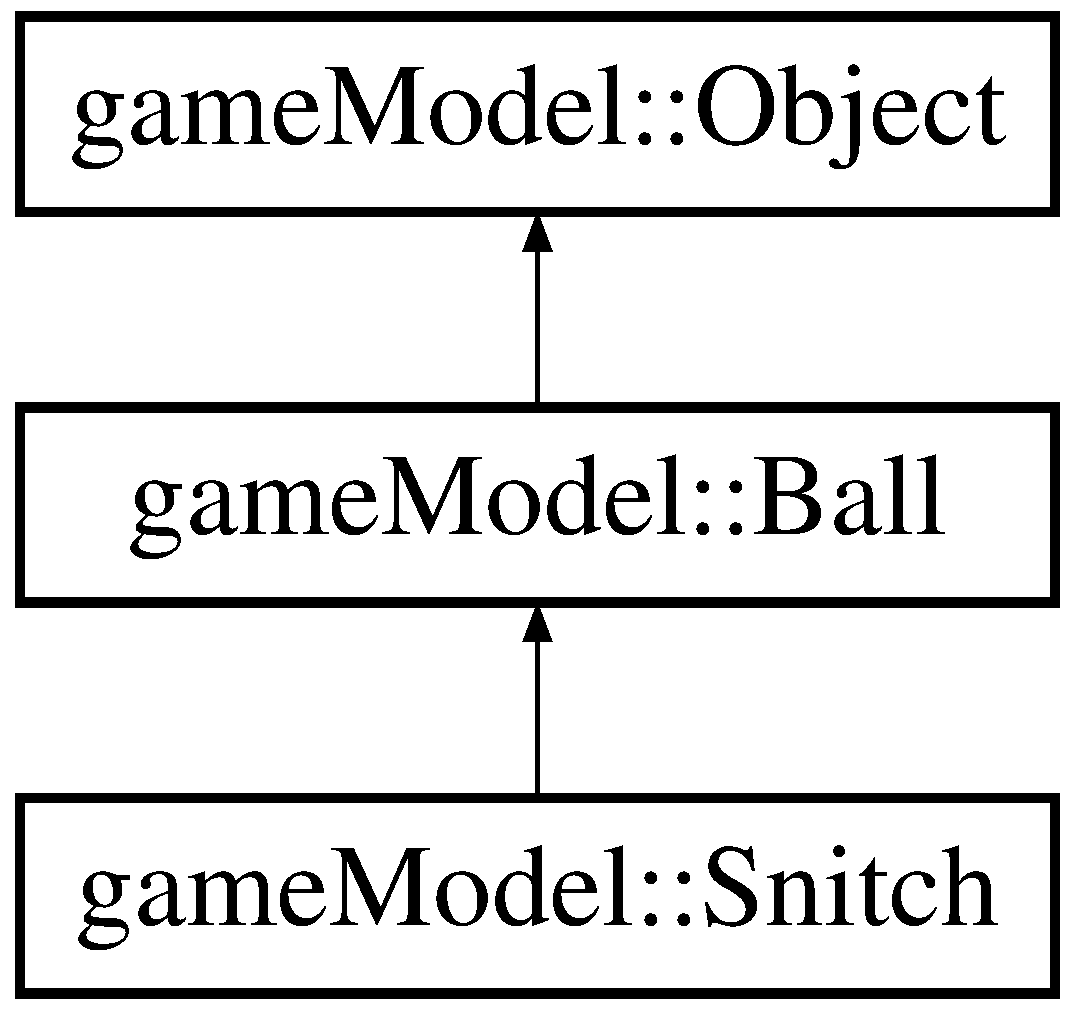
\includegraphics[height=3.000000cm]{classgame_model_1_1_snitch}
\end{center}
\end{figure}
\subsection*{Public Member Functions}
\begin{DoxyCompactItemize}
\item 
\hyperlink{classgame_model_1_1_snitch_ae0cb09809ffc99eac10821718b6de864}{Snitch} ()
\item 
\hypertarget{classgame_model_1_1_snitch_a4041553f7e9cf5b9f2ccd1fa137e6963}{{\bfseries Snitch} (\hyperlink{structgame_model_1_1_position}{Position} position)}\label{classgame_model_1_1_snitch_a4041553f7e9cf5b9f2ccd1fa137e6963}

\end{DoxyCompactItemize}
\subsection*{Data Fields}
\begin{DoxyCompactItemize}
\item 
\hypertarget{classgame_model_1_1_snitch_ad22642eb5f53c5ea7a6db2159994d47f}{bool {\bfseries exists} = false}\label{classgame_model_1_1_snitch_ad22642eb5f53c5ea7a6db2159994d47f}

\end{DoxyCompactItemize}


\subsection{Constructor \& Destructor Documentation}
\hypertarget{classgame_model_1_1_snitch_ae0cb09809ffc99eac10821718b6de864}{\index{game\-Model\-::\-Snitch@{game\-Model\-::\-Snitch}!Snitch@{Snitch}}
\index{Snitch@{Snitch}!gameModel::Snitch@{game\-Model\-::\-Snitch}}
\subsubsection[{Snitch}]{\setlength{\rightskip}{0pt plus 5cm}game\-Model\-::\-Snitch\-::\-Snitch (
\begin{DoxyParamCaption}
{}
\end{DoxyParamCaption}
)}}\label{classgame_model_1_1_snitch_ae0cb09809ffc99eac10821718b6de864}
Places \hyperlink{classgame_model_1_1_snitch}{Snitch} on random position on the field and makes it non existent 

The documentation for this class was generated from the following files\-:\begin{DoxyCompactItemize}
\item 
/home/travis/build/\-So\-Pra-\/\-Team-\/10/\-Game\-Logic/Game\-Model.\-h\item 
/home/travis/build/\-So\-Pra-\/\-Team-\/10/\-Game\-Logic/Game\-Model.\-cpp\end{DoxyCompactItemize}

\hypertarget{classgame_controller_1_1_snitch_push}{\section{game\-Controller\-:\-:Snitch\-Push Class Reference}
\label{classgame_controller_1_1_snitch_push}\index{game\-Controller\-::\-Snitch\-Push@{game\-Controller\-::\-Snitch\-Push}}
}
Inheritance diagram for game\-Controller\-:\-:Snitch\-Push\-:\begin{figure}[H]
\begin{center}
\leavevmode
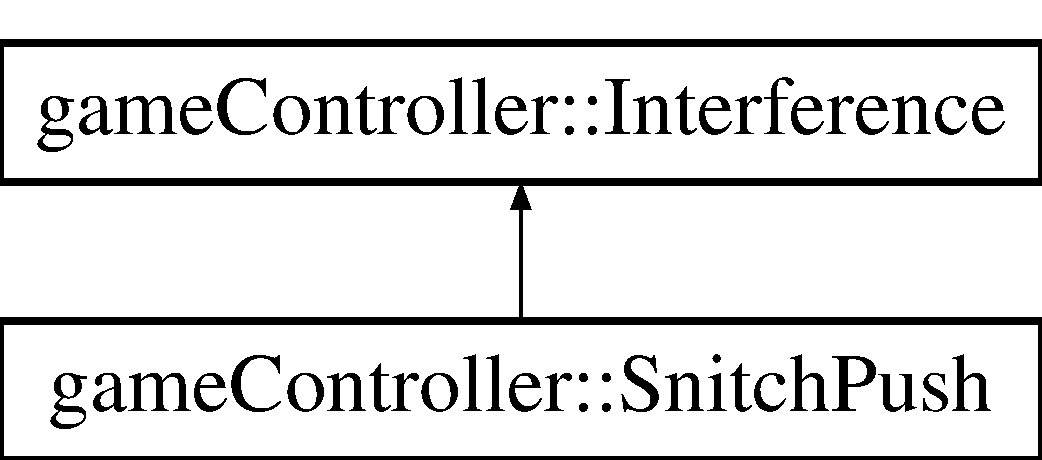
\includegraphics[height=2.000000cm]{classgame_controller_1_1_snitch_push}
\end{center}
\end{figure}
\subsection*{Public Member Functions}
\begin{DoxyCompactItemize}
\item 
\hypertarget{classgame_controller_1_1_snitch_push_ab70b837e00aeb361d84efa51dce2b97d}{{\bfseries Snitch\-Push} (std\-::shared\-\_\-ptr$<$ \hyperlink{classgame_model_1_1_environment}{game\-Model\-::\-Environment} $>$ env, std\-::shared\-\_\-ptr$<$ \hyperlink{classgame_model_1_1_team}{game\-Model\-::\-Team} $>$ team)}\label{classgame_controller_1_1_snitch_push_ab70b837e00aeb361d84efa51dce2b97d}

\item 
void \hyperlink{classgame_controller_1_1_snitch_push_a3abfb90f1d21c8b51971d75012485af4}{execute} () const override
\end{DoxyCompactItemize}
\subsection*{Additional Inherited Members}


\subsection{Member Function Documentation}
\hypertarget{classgame_controller_1_1_snitch_push_a3abfb90f1d21c8b51971d75012485af4}{\index{game\-Controller\-::\-Snitch\-Push@{game\-Controller\-::\-Snitch\-Push}!execute@{execute}}
\index{execute@{execute}!gameController::SnitchPush@{game\-Controller\-::\-Snitch\-Push}}
\subsubsection[{execute}]{\setlength{\rightskip}{0pt plus 5cm}void game\-Controller\-::\-Snitch\-Push\-::execute (
\begin{DoxyParamCaption}
{}
\end{DoxyParamCaption}
) const\hspace{0.3cm}{\ttfamily [override]}, {\ttfamily [virtual]}}}\label{classgame_controller_1_1_snitch_push_a3abfb90f1d21c8b51971d75012485af4}
Snitch is moved to random free adjacent position 

Implements \hyperlink{classgame_controller_1_1_interference_aa5ced37bf22486e1cc290bc6679c2db2}{game\-Controller\-::\-Interference}.



The documentation for this class was generated from the following files\-:\begin{DoxyCompactItemize}
\item 
/home/travis/build/\-So\-Pra-\/\-Team-\/10/\-Game\-Logic/Interference.\-h\item 
/home/travis/build/\-So\-Pra-\/\-Team-\/10/\-Game\-Logic/Interference.\-cpp\end{DoxyCompactItemize}

\hypertarget{classgame_model_1_1_team}{\section{game\-Model\-:\-:Team Class Reference}
\label{classgame_model_1_1_team}\index{game\-Model\-::\-Team@{game\-Model\-::\-Team}}
}


{\ttfamily \#include $<$Game\-Model.\-h$>$}

\subsection*{Public Member Functions}
\begin{DoxyCompactItemize}
\item 
\hyperlink{classgame_model_1_1_team_a6254ef77ea2fd282421d1508457ba53f}{Team} (const communication\-::messages\-::request\-::\-Team\-Config \&t\-Conf, communication\-::messages\-::request\-::\-Team\-Formation t\-Form, bool left\-Team)
\item 
\hypertarget{classgame_model_1_1_team_a52a305b144f89973b3500335502c0cef}{{\bfseries Team} (\hyperlink{classgame_model_1_1_seeker}{Seeker} seeker, \hyperlink{classgame_model_1_1_keeper}{Keeper} keeper, std\-::array$<$ \hyperlink{classgame_model_1_1_beater}{Beater}, 2 $>$ beaters, std\-::array$<$ \hyperlink{classgame_model_1_1_chaser}{Chaser}, 3 $>$ chasers, std\-::string name, std\-::string color\-Main, std\-::string color\-Secondary, \hyperlink{classgame_model_1_1_fanblock}{Fanblock} fanblock)}\label{classgame_model_1_1_team_a52a305b144f89973b3500335502c0cef}

\item 
auto \hyperlink{classgame_model_1_1_team_a3add38a878f50ed9a847b01d996be4ca}{get\-All\-Players} () const -\/$>$ std\-::array$<$ std\-::shared\-\_\-ptr$<$ \hyperlink{classgame_model_1_1_player}{Player} $>$, 7 $>$
\item 
bool \hyperlink{classgame_model_1_1_team_af8385c0f7f70af2aa82d082a3b6c64d3}{has\-Member} (const std\-::shared\-\_\-ptr$<$ \hyperlink{classgame_model_1_1_player}{Player} $>$ \&player) const 
\item 
int \hyperlink{classgame_model_1_1_team_aa8c1000d942a20cf9a8de559338ff869}{number\-Of\-Banned\-Members} () const 
\item 
auto \hyperlink{classgame_model_1_1_team_a1e22097a639d37333176354a83ab3038}{get\-Player\-By\-I\-D} (communication\-::messages\-::types\-::\-Entity\-Id id) const -\/$>$ std\-::optional$<$ std\-::shared\-\_\-ptr$<$ \hyperlink{classgame_model_1_1_player}{Player} $>$$>$
\end{DoxyCompactItemize}
\subsection*{Data Fields}
\begin{DoxyCompactItemize}
\item 
\hypertarget{classgame_model_1_1_team_a302e269f8d6d272ca2c56f3167daf39b}{std\-::shared\-\_\-ptr$<$ \hyperlink{classgame_model_1_1_seeker}{Seeker} $>$ {\bfseries seeker}}\label{classgame_model_1_1_team_a302e269f8d6d272ca2c56f3167daf39b}

\item 
\hypertarget{classgame_model_1_1_team_a425f35bd2eb0fbb8b284515ef98b2c7c}{std\-::shared\-\_\-ptr$<$ \hyperlink{classgame_model_1_1_keeper}{Keeper} $>$ {\bfseries keeper}}\label{classgame_model_1_1_team_a425f35bd2eb0fbb8b284515ef98b2c7c}

\item 
\hypertarget{classgame_model_1_1_team_a0636cb95d07be8501aaf13f80d5a20d9}{std\-::array$<$ std\-::shared\-\_\-ptr\\*
$<$ \hyperlink{classgame_model_1_1_beater}{Beater} $>$, 2 $>$ {\bfseries beaters}}\label{classgame_model_1_1_team_a0636cb95d07be8501aaf13f80d5a20d9}

\item 
\hypertarget{classgame_model_1_1_team_afea41de9c9b5871774ea140f6e14bbdc}{std\-::array$<$ std\-::shared\-\_\-ptr\\*
$<$ \hyperlink{classgame_model_1_1_chaser}{Chaser} $>$, 3 $>$ {\bfseries chasers}}\label{classgame_model_1_1_team_afea41de9c9b5871774ea140f6e14bbdc}

\item 
\hypertarget{classgame_model_1_1_team_a8a60b80727b62710d62506792f955e1f}{const std\-::string {\bfseries name}}\label{classgame_model_1_1_team_a8a60b80727b62710d62506792f955e1f}

\item 
\hypertarget{classgame_model_1_1_team_a4b47c344630336be16e749104527c8e4}{const std\-::string {\bfseries color\-Main}}\label{classgame_model_1_1_team_a4b47c344630336be16e749104527c8e4}

\item 
\hypertarget{classgame_model_1_1_team_a53adedaa19dd76d2a244e4ed4f641012}{const std\-::string {\bfseries color\-Secondary}}\label{classgame_model_1_1_team_a53adedaa19dd76d2a244e4ed4f641012}

\item 
\hypertarget{classgame_model_1_1_team_a1b3329955b8b3bde885f8ee8f0029213}{int {\bfseries score} \{\}}\label{classgame_model_1_1_team_a1b3329955b8b3bde885f8ee8f0029213}

\item 
\hypertarget{classgame_model_1_1_team_a89c473adc822535d64c38db6637c4eb2}{\hyperlink{classgame_model_1_1_fanblock}{Fanblock} {\bfseries fanblock}}\label{classgame_model_1_1_team_a89c473adc822535d64c38db6637c4eb2}

\end{DoxyCompactItemize}


\subsection{Detailed Description}
Represents a \hyperlink{classgame_model_1_1_team}{Team} 

\subsection{Constructor \& Destructor Documentation}
\hypertarget{classgame_model_1_1_team_a6254ef77ea2fd282421d1508457ba53f}{\index{game\-Model\-::\-Team@{game\-Model\-::\-Team}!Team@{Team}}
\index{Team@{Team}!gameModel::Team@{game\-Model\-::\-Team}}
\subsubsection[{Team}]{\setlength{\rightskip}{0pt plus 5cm}game\-Model\-::\-Team\-::\-Team (
\begin{DoxyParamCaption}
\item[{const communication\-::messages\-::request\-::\-Team\-Config \&}]{t\-Conf, }
\item[{communication\-::messages\-::request\-::\-Team\-Formation}]{t\-Form, }
\item[{bool}]{left\-Team}
\end{DoxyParamCaption}
)}}\label{classgame_model_1_1_team_a6254ef77ea2fd282421d1508457ba53f}
Constructs a \hyperlink{classgame_model_1_1_team}{Team} from server config types 
\begin{DoxyParams}{Parameters}
{\em left\-Team} & select if team si on left or right side \\
\hline
\end{DoxyParams}


\subsection{Member Function Documentation}
\hypertarget{classgame_model_1_1_team_a3add38a878f50ed9a847b01d996be4ca}{\index{game\-Model\-::\-Team@{game\-Model\-::\-Team}!get\-All\-Players@{get\-All\-Players}}
\index{get\-All\-Players@{get\-All\-Players}!gameModel::Team@{game\-Model\-::\-Team}}
\subsubsection[{get\-All\-Players}]{\setlength{\rightskip}{0pt plus 5cm}auto game\-Model\-::\-Team\-::get\-All\-Players (
\begin{DoxyParamCaption}
{}
\end{DoxyParamCaption}
) const -\/$>$ std\-::array$<$std\-::shared\-\_\-ptr$<${\bf Player}$>$, 7$>$}}\label{classgame_model_1_1_team_a3add38a878f50ed9a847b01d996be4ca}
gets all Players of the team \begin{DoxyReturn}{Returns}

\end{DoxyReturn}
\hypertarget{classgame_model_1_1_team_a1e22097a639d37333176354a83ab3038}{\index{game\-Model\-::\-Team@{game\-Model\-::\-Team}!get\-Player\-By\-I\-D@{get\-Player\-By\-I\-D}}
\index{get\-Player\-By\-I\-D@{get\-Player\-By\-I\-D}!gameModel::Team@{game\-Model\-::\-Team}}
\subsubsection[{get\-Player\-By\-I\-D}]{\setlength{\rightskip}{0pt plus 5cm}auto game\-Model\-::\-Team\-::get\-Player\-By\-I\-D (
\begin{DoxyParamCaption}
\item[{communication\-::messages\-::types\-::\-Entity\-Id}]{id}
\end{DoxyParamCaption}
) const -\/$>$ std\-::optional$<$std\-::shared\-\_\-ptr$<${\bf Player}$>$$>$}}\label{classgame_model_1_1_team_a1e22097a639d37333176354a83ab3038}
Get player by server entity ids 
\begin{DoxyParams}{Parameters}
{\em id} & \\
\hline
\end{DoxyParams}
\begin{DoxyReturn}{Returns}

\end{DoxyReturn}
\hypertarget{classgame_model_1_1_team_af8385c0f7f70af2aa82d082a3b6c64d3}{\index{game\-Model\-::\-Team@{game\-Model\-::\-Team}!has\-Member@{has\-Member}}
\index{has\-Member@{has\-Member}!gameModel::Team@{game\-Model\-::\-Team}}
\subsubsection[{has\-Member}]{\setlength{\rightskip}{0pt plus 5cm}bool game\-Model\-::\-Team\-::has\-Member (
\begin{DoxyParamCaption}
\item[{const std\-::shared\-\_\-ptr$<$ {\bf Player} $>$ \&}]{player}
\end{DoxyParamCaption}
) const}}\label{classgame_model_1_1_team_af8385c0f7f70af2aa82d082a3b6c64d3}
Determins wether a given player is a member of the team 
\begin{DoxyParams}{Parameters}
{\em player} & \\
\hline
\end{DoxyParams}
\begin{DoxyReturn}{Returns}
true if player is a member of the team. false otherwise 
\end{DoxyReturn}
\hypertarget{classgame_model_1_1_team_aa8c1000d942a20cf9a8de559338ff869}{\index{game\-Model\-::\-Team@{game\-Model\-::\-Team}!number\-Of\-Banned\-Members@{number\-Of\-Banned\-Members}}
\index{number\-Of\-Banned\-Members@{number\-Of\-Banned\-Members}!gameModel::Team@{game\-Model\-::\-Team}}
\subsubsection[{number\-Of\-Banned\-Members}]{\setlength{\rightskip}{0pt plus 5cm}int game\-Model\-::\-Team\-::number\-Of\-Banned\-Members (
\begin{DoxyParamCaption}
{}
\end{DoxyParamCaption}
) const}}\label{classgame_model_1_1_team_aa8c1000d942a20cf9a8de559338ff869}
gets the number of banned players in the team 

The documentation for this class was generated from the following files\-:\begin{DoxyCompactItemize}
\item 
/home/travis/build/\-So\-Pra-\/\-Team-\/10/\-Game\-Logic/Game\-Model.\-h\item 
/home/travis/build/\-So\-Pra-\/\-Team-\/10/\-Game\-Logic/Game\-Model.\-cpp\end{DoxyCompactItemize}

\hypertarget{classgame_controller_1_1_teleport}{\section{game\-Controller\-:\-:Teleport Class Reference}
\label{classgame_controller_1_1_teleport}\index{game\-Controller\-::\-Teleport@{game\-Controller\-::\-Teleport}}
}
Inheritance diagram for game\-Controller\-:\-:Teleport\-:\begin{figure}[H]
\begin{center}
\leavevmode
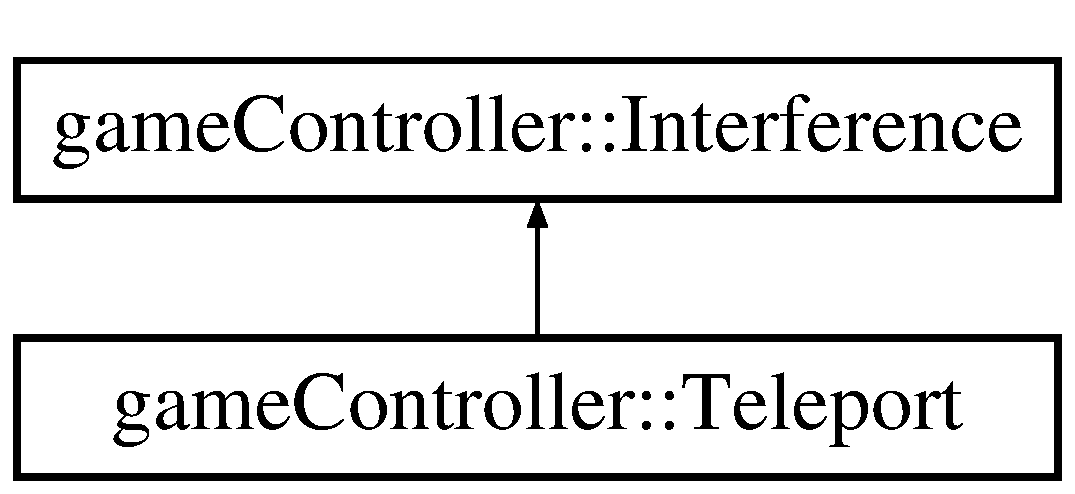
\includegraphics[height=2.000000cm]{classgame_controller_1_1_teleport}
\end{center}
\end{figure}
\subsection*{Public Member Functions}
\begin{DoxyCompactItemize}
\item 
\hypertarget{classgame_controller_1_1_teleport_ad427f67456586b006eb15142a96435df}{{\bfseries Teleport} (std\-::shared\-\_\-ptr$<$ \hyperlink{classgame_model_1_1_environment}{game\-Model\-::\-Environment} $>$ env, std\-::shared\-\_\-ptr$<$ \hyperlink{classgame_model_1_1_team}{game\-Model\-::\-Team} $>$ team, std\-::shared\-\_\-ptr$<$ \hyperlink{classgame_model_1_1_player}{game\-Model\-::\-Player} $>$ target)}\label{classgame_controller_1_1_teleport_ad427f67456586b006eb15142a96435df}

\item 
void \hyperlink{classgame_controller_1_1_teleport_a9e10c37934bf7447f1cee64545fbf138}{execute} () const override
\end{DoxyCompactItemize}
\subsection*{Additional Inherited Members}


\subsection{Member Function Documentation}
\hypertarget{classgame_controller_1_1_teleport_a9e10c37934bf7447f1cee64545fbf138}{\index{game\-Controller\-::\-Teleport@{game\-Controller\-::\-Teleport}!execute@{execute}}
\index{execute@{execute}!gameController::Teleport@{game\-Controller\-::\-Teleport}}
\subsubsection[{execute}]{\setlength{\rightskip}{0pt plus 5cm}void game\-Controller\-::\-Teleport\-::execute (
\begin{DoxyParamCaption}
{}
\end{DoxyParamCaption}
) const\hspace{0.3cm}{\ttfamily [override]}, {\ttfamily [virtual]}}}\label{classgame_controller_1_1_teleport_a9e10c37934bf7447f1cee64545fbf138}
Teleports target player to random free location on the field 

Implements \hyperlink{classgame_controller_1_1_interference_aa5ced37bf22486e1cc290bc6679c2db2}{game\-Controller\-::\-Interference}.



The documentation for this class was generated from the following files\-:\begin{DoxyCompactItemize}
\item 
/home/travis/build/\-So\-Pra-\/\-Team-\/10/\-Game\-Logic/Interference.\-h\item 
/home/travis/build/\-So\-Pra-\/\-Team-\/10/\-Game\-Logic/Interference.\-cpp\end{DoxyCompactItemize}

\hypertarget{structgame_model_1_1_timeouts}{\section{game\-Model\-:\-:Timeouts Struct Reference}
\label{structgame_model_1_1_timeouts}\index{game\-Model\-::\-Timeouts@{game\-Model\-::\-Timeouts}}
}


{\ttfamily \#include $<$Game\-Model.\-h$>$}

\subsection*{Data Fields}
\begin{DoxyCompactItemize}
\item 
\hypertarget{structgame_model_1_1_timeouts_aa98e3131cb2b9c69a16fcac3fb34ce9e}{int {\bfseries player\-Turn}}\label{structgame_model_1_1_timeouts_aa98e3131cb2b9c69a16fcac3fb34ce9e}

\item 
\hypertarget{structgame_model_1_1_timeouts_a1645cb3220ee94d55ec2ceba7a34054c}{int {\bfseries fan\-Turn}}\label{structgame_model_1_1_timeouts_a1645cb3220ee94d55ec2ceba7a34054c}

\item 
\hypertarget{structgame_model_1_1_timeouts_a4b09c9deeb9c584b0d36a4ec79f18ba4}{int {\bfseries player\-Phase}}\label{structgame_model_1_1_timeouts_a4b09c9deeb9c584b0d36a4ec79f18ba4}

\item 
\hypertarget{structgame_model_1_1_timeouts_a00fe919f0c92bb2e96807b8aea6cf308}{int {\bfseries fan\-Phase}}\label{structgame_model_1_1_timeouts_a00fe919f0c92bb2e96807b8aea6cf308}

\item 
\hypertarget{structgame_model_1_1_timeouts_a38e03ad300283aaad1ea1f4d3d6fb646}{int {\bfseries ball\-Phase}}\label{structgame_model_1_1_timeouts_a38e03ad300283aaad1ea1f4d3d6fb646}

\end{DoxyCompactItemize}


\subsection{Detailed Description}
All different kinds of time limits and timeouts 

The documentation for this struct was generated from the following file\-:\begin{DoxyCompactItemize}
\item 
/home/travis/build/\-So\-Pra-\/\-Team-\/10/\-Game\-Logic/Game\-Model.\-h\end{DoxyCompactItemize}

\hypertarget{classgame_model_1_1_vector}{\section{game\-Model\-:\-:Vector Class Reference}
\label{classgame_model_1_1_vector}\index{game\-Model\-::\-Vector@{game\-Model\-::\-Vector}}
}
\subsection*{Public Member Functions}
\begin{DoxyCompactItemize}
\item 
\hyperlink{classgame_model_1_1_vector_abfcad404f21198136afc5c8e8b820639}{Vector} (double \hyperlink{classgame_model_1_1_vector_a739e0039692645e340238e9154be214a}{x}, double \hyperlink{classgame_model_1_1_vector_a34f020c4e0e747a90002bb53d643a55c}{y})
\item 
\hypertarget{classgame_model_1_1_vector_a00a388626afcfefb1ab1bb22706863b0}{{\bfseries Vector} (const \hyperlink{structgame_model_1_1_position}{Position} \&p1, const \hyperlink{structgame_model_1_1_position}{Position} \&p2)}\label{classgame_model_1_1_vector_a00a388626afcfefb1ab1bb22706863b0}

\item 
double \hyperlink{classgame_model_1_1_vector_a3d4c4a7cce251f2522271891b23551ab}{abs} () const 
\item 
void \hyperlink{classgame_model_1_1_vector_ade91c1e7810dad34c4cbda5d87ad275f}{normalize} ()
\item 
\hypertarget{classgame_model_1_1_vector_a015dc4960d65f384dab4f11c2b3418f7}{bool {\bfseries operator==} (const \hyperlink{classgame_model_1_1_vector}{Vector} \&v) const }\label{classgame_model_1_1_vector_a015dc4960d65f384dab4f11c2b3418f7}

\item 
\hypertarget{classgame_model_1_1_vector_a365b826d3195eb95b9b2b81cbb13d26a}{\hyperlink{classgame_model_1_1_vector}{Vector} {\bfseries operator$\ast$} (const double \&c) const }\label{classgame_model_1_1_vector_a365b826d3195eb95b9b2b81cbb13d26a}

\item 
\hypertarget{classgame_model_1_1_vector_ac3a756df6a0cfe4811e1c2935507d910}{\hyperlink{classgame_model_1_1_vector}{Vector} {\bfseries operator+} (const \hyperlink{classgame_model_1_1_vector}{Vector} \&v) const }\label{classgame_model_1_1_vector_ac3a756df6a0cfe4811e1c2935507d910}

\item 
\hypertarget{classgame_model_1_1_vector_ad15455e6cf880d7f00586a66337d1b8b}{\hyperlink{structgame_model_1_1_position}{Position} {\bfseries operator+} (const \hyperlink{structgame_model_1_1_position}{Position} \&p) const }\label{classgame_model_1_1_vector_ad15455e6cf880d7f00586a66337d1b8b}

\end{DoxyCompactItemize}
\subsection*{Data Fields}
\begin{DoxyCompactItemize}
\item 
\hypertarget{classgame_model_1_1_vector_a739e0039692645e340238e9154be214a}{double \hyperlink{classgame_model_1_1_vector_a739e0039692645e340238e9154be214a}{x}}\label{classgame_model_1_1_vector_a739e0039692645e340238e9154be214a}

\begin{DoxyCompactList}\small\item\em x component of the vector. \end{DoxyCompactList}\item 
\hypertarget{classgame_model_1_1_vector_a34f020c4e0e747a90002bb53d643a55c}{double \hyperlink{classgame_model_1_1_vector_a34f020c4e0e747a90002bb53d643a55c}{y}}\label{classgame_model_1_1_vector_a34f020c4e0e747a90002bb53d643a55c}

\begin{DoxyCompactList}\small\item\em y component of the vector. \end{DoxyCompactList}\end{DoxyCompactItemize}


\subsection{Constructor \& Destructor Documentation}
\hypertarget{classgame_model_1_1_vector_abfcad404f21198136afc5c8e8b820639}{\index{game\-Model\-::\-Vector@{game\-Model\-::\-Vector}!Vector@{Vector}}
\index{Vector@{Vector}!gameModel::Vector@{game\-Model\-::\-Vector}}
\subsubsection[{Vector}]{\setlength{\rightskip}{0pt plus 5cm}game\-Model\-::\-Vector\-::\-Vector (
\begin{DoxyParamCaption}
\item[{double}]{x, }
\item[{double}]{y}
\end{DoxyParamCaption}
)}}\label{classgame_model_1_1_vector_abfcad404f21198136afc5c8e8b820639}
main constructor for the vector. 
\begin{DoxyParams}{Parameters}
{\em x} & x component of the vector. \\
\hline
{\em y} & y component of the vector. \\
\hline
\end{DoxyParams}


\subsection{Member Function Documentation}
\hypertarget{classgame_model_1_1_vector_a3d4c4a7cce251f2522271891b23551ab}{\index{game\-Model\-::\-Vector@{game\-Model\-::\-Vector}!abs@{abs}}
\index{abs@{abs}!gameModel::Vector@{game\-Model\-::\-Vector}}
\subsubsection[{abs}]{\setlength{\rightskip}{0pt plus 5cm}double game\-Model\-::\-Vector\-::abs (
\begin{DoxyParamCaption}
{}
\end{DoxyParamCaption}
) const}}\label{classgame_model_1_1_vector_a3d4c4a7cce251f2522271891b23551ab}
get the euclidean norm of the vector. \begin{DoxyReturn}{Returns}
the euclidean norm as double. 
\end{DoxyReturn}
\hypertarget{classgame_model_1_1_vector_ade91c1e7810dad34c4cbda5d87ad275f}{\index{game\-Model\-::\-Vector@{game\-Model\-::\-Vector}!normalize@{normalize}}
\index{normalize@{normalize}!gameModel::Vector@{game\-Model\-::\-Vector}}
\subsubsection[{normalize}]{\setlength{\rightskip}{0pt plus 5cm}void game\-Model\-::\-Vector\-::normalize (
\begin{DoxyParamCaption}
{}
\end{DoxyParamCaption}
)}}\label{classgame_model_1_1_vector_ade91c1e7810dad34c4cbda5d87ad275f}
normalize the vector. 

The documentation for this class was generated from the following files\-:\begin{DoxyCompactItemize}
\item 
/home/travis/build/\-So\-Pra-\/\-Team-\/10/\-Game\-Logic/Game\-Model.\-h\item 
/home/travis/build/\-So\-Pra-\/\-Team-\/10/\-Game\-Logic/Game\-Model.\-cpp\end{DoxyCompactItemize}

%--- End generated contents ---

% Index
\newpage
\phantomsection
\addcontentsline{toc}{chapter}{Index}
\printindex

\end{document}
